\Chapter{ARTICLE 1: PERFORMANCE ANALYSIS USING AUTOMATIC GROUPING}\label{sec:Theme2}
\textbf{Authors}\\
Isnaldo Francisco de Melo Junior\\
École Polytechnique de Montréal\\
Isnaldo-francisco.de-melo-junior@polymtl.ca\\
 
Michel Dagenais\\
École Polytechnique de Montréal\\
michel.dagenais@polymtl.ca\\
 
\textbf{Index terms} – Performance analysis, Tracing, Software visualization, Heuristic, Groups.\\

\section{Abstract}
\label{sec:abstract}
Performance has become more important on software development and maintenance. To address this concern, teams of developers use tracing tools to improve the performance or track performance related bugs. On this work we developed an automated technique to find the cause of performance issues, which do not require deep knowledge of the system. This approach is capable to indicate the performance cause using a comparative methodology on slow and fast executions. We applied the solution on some use cases and were able to find the specific cause of them. Also, we implemented the solution on a framework to help developers on similar problems together with a differential flame graph tool.


\section{Introduction}
\label{sec:introduction}
Software performance is a major concern for software development. Various studies highlight the use of tools as debugging and tracing to help on performance problems, which can be used to improve performance or detect performance issues.
% The problem
One example of performance issue is the comparison of similar executions of the same program in the same configuration setting. An example was found in \cite{doray_article}, after executing several times the same query operation on MongoDB, a free open-source database framework, its performance decreases abruptly a further investigation lead to the root cause of this performance issue.

% The solutions
For this kind of performance problem, which is related with the execution inside a real system, the current solutions are to debug or to trace it. The first one, debugging, is the location of code and wrong executions directly on the source by execution the code in a locked environment using breakpoints. However, some debugging tools require the reproduction of the exactly issue to trigger the same code mechanism and its necessary to retard the execution of the program while doing this process.

On the other hand, a trace is an execution log of a software that consists essentially of an ordered list of events. An event is generated when a certain path of the code is executed, commonly denominated tracepoint, where each event consists of a timestamp, a type and some arbitrary payload \cite{francis1}. tracepoints can be embedded on the code in two ways: statically or dynamically inserted. The later, dynamic tracing, gives the possibility to add tracepoints without modifying the source code and the sooner requires the modification of the source code. Besides, tracing can be performed at the kernel and user-space level \cite{francis1}.\\

Unlike debugging, it is possible to trace a program without interrupt it, yet, there is an overhead caused by its usage. A good tracer needs to minimize the disturbance of the running program to be a useful tool for analysis. LTTng\cite{desnoyers}, developed by Mathieu Desnoyers, has this minimal level of impact on the system and consequently allows to trace the user-space and the kernel space with minimal interference. LTTng, allows the analysis of task interactions with each other and with the operating system. Locating and analyzing performance problems is not a trivial activity because of their large size, since more events generate more information to be gathered and analyzed. 

After collecting the data on the tracer, it is necessary to analyze the software behaviour through some mechanism, for instance the call graph \cite{call_graph}. A call graph is a representation of the stack frames of the software and can be built using different techniques. This analysis requires expert knowledge and deep analysis of the system since this process was not automated yet.

Through tracing mechanisms is possible to build a dynamic model of the software or, in other words, a calling tree of it. Moreover, tracing allows the possibility to add performance measurements to this structure, as shown in \cite{doray_article}.

In summary, from the enhanced data structure described above and considering the lack of an automate solution to solve problems as the stated above, it is possible to build a solution that records several software properties at run time. Moreover, using some specific grouping mechanisms it is possible to find root causes of several performance issues using this comparative approach.\\

This paper introduces an automated solution for clustering metrics using the call context tree to find performance related issues. We implemented it on TraceCompass with visualization mechanisms to facilitate the analysis of different aspects of the Calling Context Tree. Then we applied this technique on four different use cases to analyze the performance problem of them. Finally, we discuss the drawbacks of this technique and the possible solutions to overcome them aiming to apply this analysis on real software.

The research aims to investigate the following research questions;

\begin{itemize}
\item RQ 1: How can we build an efficient and flexible model for performance comparison?
\item RQ 2: How to automate the performance analysis on several runs using performance counters?
% \item RQ 3: The root cause found using the approach is accurate?
\item RQ 3: How accurate was the obtained results ?
\end{itemize}

\textbf{This paper is organized as follows} The related work is presented in section \ref{sec:related-work}, then the solution is presented in \ref{sec:solution} with the clustering technique. In section \ref{sec:methodology}, we present the methodology used followed by the micro-benchmarks and an illustrative example of the analysis. The use case section \ref{sec:usecases}, the discussion of the results \ref{sec:results} and a section with some limitations \ref{sec:validity}. Finally the conclusion \ref{sec:conclusion},

 
\section{Related Work}
\label{sec:related-work}

%Specifically considering the approach used here, comparing the metrics of a program to classify them the work of Francois Doray, in TraceCompare has a similar approach.
In this section will be presented the basic principles of current tools used to find performance issues. The related work was divided in: Data collection, Analysis tools and Visualization tools that are described below.\\

% \textbf{Data collection}\\
From the perspectives of Data Collection, there are two main works related to this work, LTTng and Linux Perf Events.

% \subsection{LTTng}
The first, LTTng, Linux Trace Toolkit Next Generation \cite{desnoyers}, tracer can record events from the Linux kernel and from user space applications into a single trace. It is also designed to have a minimal overhead on traced systems. It is therefore well suited to our goal of collecting all the factors that contribute to the execution time of tasks in production environment.\\

% \subsection{Linux Perf}
The second, Linux Perf Events is a profiler tool for Linux 2.6+ based systems that abstracts away CPU hardware differences in Linux performance measurements and presents a simple command-line interface. Perf is based on the perf events interface exported by recent versions of the Linux kernel. This article demonstrates the perf tool through example runs \cite{perf}. It is possible to record software events and hardware events \cite{vitillo}.\\
It is interesting to highlight that the Perf tool can be used to record profiles on per-thread, per-process and per-cpu basis \cite{perftool}.\\
% \textbf{Analysis tools}\\
From the point of view of Analysis tool, there are two main tools related to this work, TraceCompare and Trevis.
% \subsection{TraceCompare}
The first tool, TraceCompare, was developed in Dorsal lab \cite{tracecompare}, which creates an enhanced Calling Context Tree to measure the metrics from specific segments of a trace. Those segments are defined by the user as sequences of begin and end. This tool was developed to compare traces of execution and it uses a javascript front-end and tibeebeetles as back-end. To do this CPU profiling comparison, the GUI tools provides a Differential flame graphs as defined in \cite{differential_flame}.
 It was able to find abnormalities in the write function of MongoDB after several runs. However, TraceCompare requires expert knowledge and also some statically metrics of analysis \cite{doray_thesis}.\\
% \subsection{Trevis}
The second tool, from Lugano University, Trevis \cite{trevis}, is a visualization and also an analysis framework. It was developed to study the CCT produced another tool called FlyBy software. Like TraceCompare, it relies on a calling context tree, CCT, on the caller-callee relationship. Trevis is a visualization and analysis framework that 
allows the users to play with the CCTs by applying several methods.
However, this tool relies in a human interaction, which occurs at FlyBy, to stipulate on the slower executions. FlyBy provides after an report of failure containing this information that later can be used in Trevis to be analyzed.\\
% \subsection{Spectroscope}
The third tool, Spectroscope, was developed in \cite{Sambasivan2011DPC19724571972463}, that is a tool that uses statistical and high level analysis, in fact, it was design to find changes in behaviour, not find specific anomalies and it was used to find problems in two versions (or periods) on Google's Ursa Minor distributed software. Specifically for this software, five problems are described. It uses Startdust as end-to-end tracers and it added some overhead on Ursa Minor performance, depending the operation. \\
It uses Perl language and MATLAB statistical comparison of no problematic period and a problematic period, also using DOT for the plotting part.
The statical comparison used is the Kolomogrov-Smirnov test,  which is a non-parametric test for mutation identification that compares the shapes and distribution of mathematical function and later using a ranking system for mutation identification.\\
 Spectroscope uses normalized discounted cumulative gain (NDCG), for the performance evaluation is used a range evaluation. Spectroscope is similar with Pip in \cite{Pip} and TAU in \cite{TAU}.\\
% \subsection{Introperf}
Finally, Introperf developed by \cite{Introperf} is a tool that uses system stack traces to generate CCT, called Performance Annotated CCT that they call PA-CCT. Then, it ranks the latencies and compare them \cite{Introperf}. The intend of this tool is to be used in a post-development stage. It was implemented using ETW, \cite{ETW}. It is explained on the paper about the latency inference algorithm used for this calculation. They used this approach to to avoid the requirement of source code or modification to application. \\

% \textbf{Visualization tools}\\
% \subsection{Flame Graph}
From the point of visualization of comparison technique, the flame graphs and differential flame graphs, developed by Brendan Gregg is a very popular technique. They can be used for comparing the executions, it is possible to use a Flame Graph diagram. As defined by Brendan Gregg \cite{differential_flame}, Differential Flame Graphs can be a useful tool for comparing executions. A Differential Flame Graph is a visualization technique highlight differences on collections of stack traces (aka call stacks), from two different executions. Flame graphs are commonly used to visualize CPU profiler output, where stack traces are collected using sampling.


\section{Motivation}
\label{sec:motivation}
The main motivation for this research was the current limitations of the current tools to track problems on executions that does not appear often, for example one execution long run among a thousand that work perfectly. 
This difficult relies mainly on the amount of data that is needed to be generated and analyzed comparatively. 

From the point of view of the grouping techniques, the current more reliable technique still require some human analysis of the data, which would consume time and undermine an automated technique. This is the reason for the development of the auto grouping technique, which combines an heuristic evaluation.


The implementation also developed the RGG differential flamegraph to compare groups of executions. This implementation uses a three colors: red, green and gray. This was necessary to avoid the ambiguity that the original work developed by Brendan Gregg gave, where the green color could mean faster execution or equal execution, in a comparative way.

This methodology developed can be applied in other scenarios and it is independent from the implementation. Besides it is also independent from the grouping algorithm, since it is an heuristic and not an algorithm. Combined with the Apriori algorithm, the grouping technique can provide strong insights on complex cases.

Finally the motivation to implement the solution in TraceCompass is because of its reliability as trace framework. TraceCompass is currently supported by Ericsson Inc. and Dorsal lab at Polytechnique Montreal, and has several features, which combined, form a complete analysis framework for different kinds of traces.

\section{Solution}
\label{sec:solution}
On this section, we discuss about the solution developed, starting from the data structure, which the work relies, then the algorithms used to do the grouping mechanism, then the cluster algorithm and the overall methodology. \\

  The methodology can be summarized in the following process:\\
  First, we trace a program using statically or dynamically embedded tracepoints. Then we read the tracing and develop a CCT recording, also the performance metrics. Later, we run the clustering techniques and the association rule, which indicated the possible cause of the performance issue.
  
    \subsubsection{Recording of execution}
    We record the program executing using LTTng, this tracer has low overhead, therefore is adequate for this type of research. 
    The trace is also recorded with the performance metrics such as instructions, cache-misses, page-faults, and schedule switches by using the perf counters tools in Linux.
    
    \subsubsection{Generating the data structure}
    After the recording in different scenarios, a pre-processing of building a structure for comparison is done, this structure is a enhanced calling context tree. 
    To do this process, we use trace compare to divide the tracing in segments, delimited using: e.g. in the case of sys\_open, we used systemCallOpen and systemCallExit.
    In this process we aim to construct comparable information using ECCT (or EDT), which each node represent a call and the information in this call will be within the nodes. A delta of the entry and the exit for each metric is recorded in the node, in a sampling scheme.
    
    \subsubsection{Clustering technique}
    After the data was pre-processed and the tree is built, a mathematical model is done and its behaviour compared to its input can be determined. 
    
    \subsubsection{Execution Comparison}
    With the groups divided the next phase is the comparison among them. There are possible to ways to compare the groups: compare the mean and median for each group or use the Apriori Association described in section \ref{sec:association}.
    
\subsection{Data Structure}
% \textit{Call Graph}\\
%     The call graph is a useful data representation for control and data flow programs which investigate interprocedural communication (i.e., how procedures exchange information). It contains all the relationships among the procedures in a program and can contain auxiliary information concerning the
%     data within each procedure and global data shared among procedures \cite{call_graph}.

\textit{Calling Context Tree}\\
Calling contexts are very important for a wide range of applications such as profiling, debugging, and event logging. Most applications perform expensive \textit{stack walking} to recover contexts\cite{precise}. The resulting contexts are often explicitly represented as a sequence of call sites and hence bulky. The goal of calling context encoding is to uniquely represent the current context of any execution point using a small number of integer identifiers (IDs). This data structure was introduced by \cite{27} and reused by \cite{4}, \cite{28}.
% \textit{Enhanced Calling Context Tree}\\
    In this work we aggregate data, related to the performance on the Calling Context Tree, which gives the concept of enhanced structure. The aggregated data is related with the performance metrics, the data is added in the tree nodes and gives the possibility to be analyzed off-line.
    The Figure \ref{fig:ecct_dt} demonstrates the difference between the dynamic tree and the calling context tree.
    \begin{figure}[h]
        \centering
        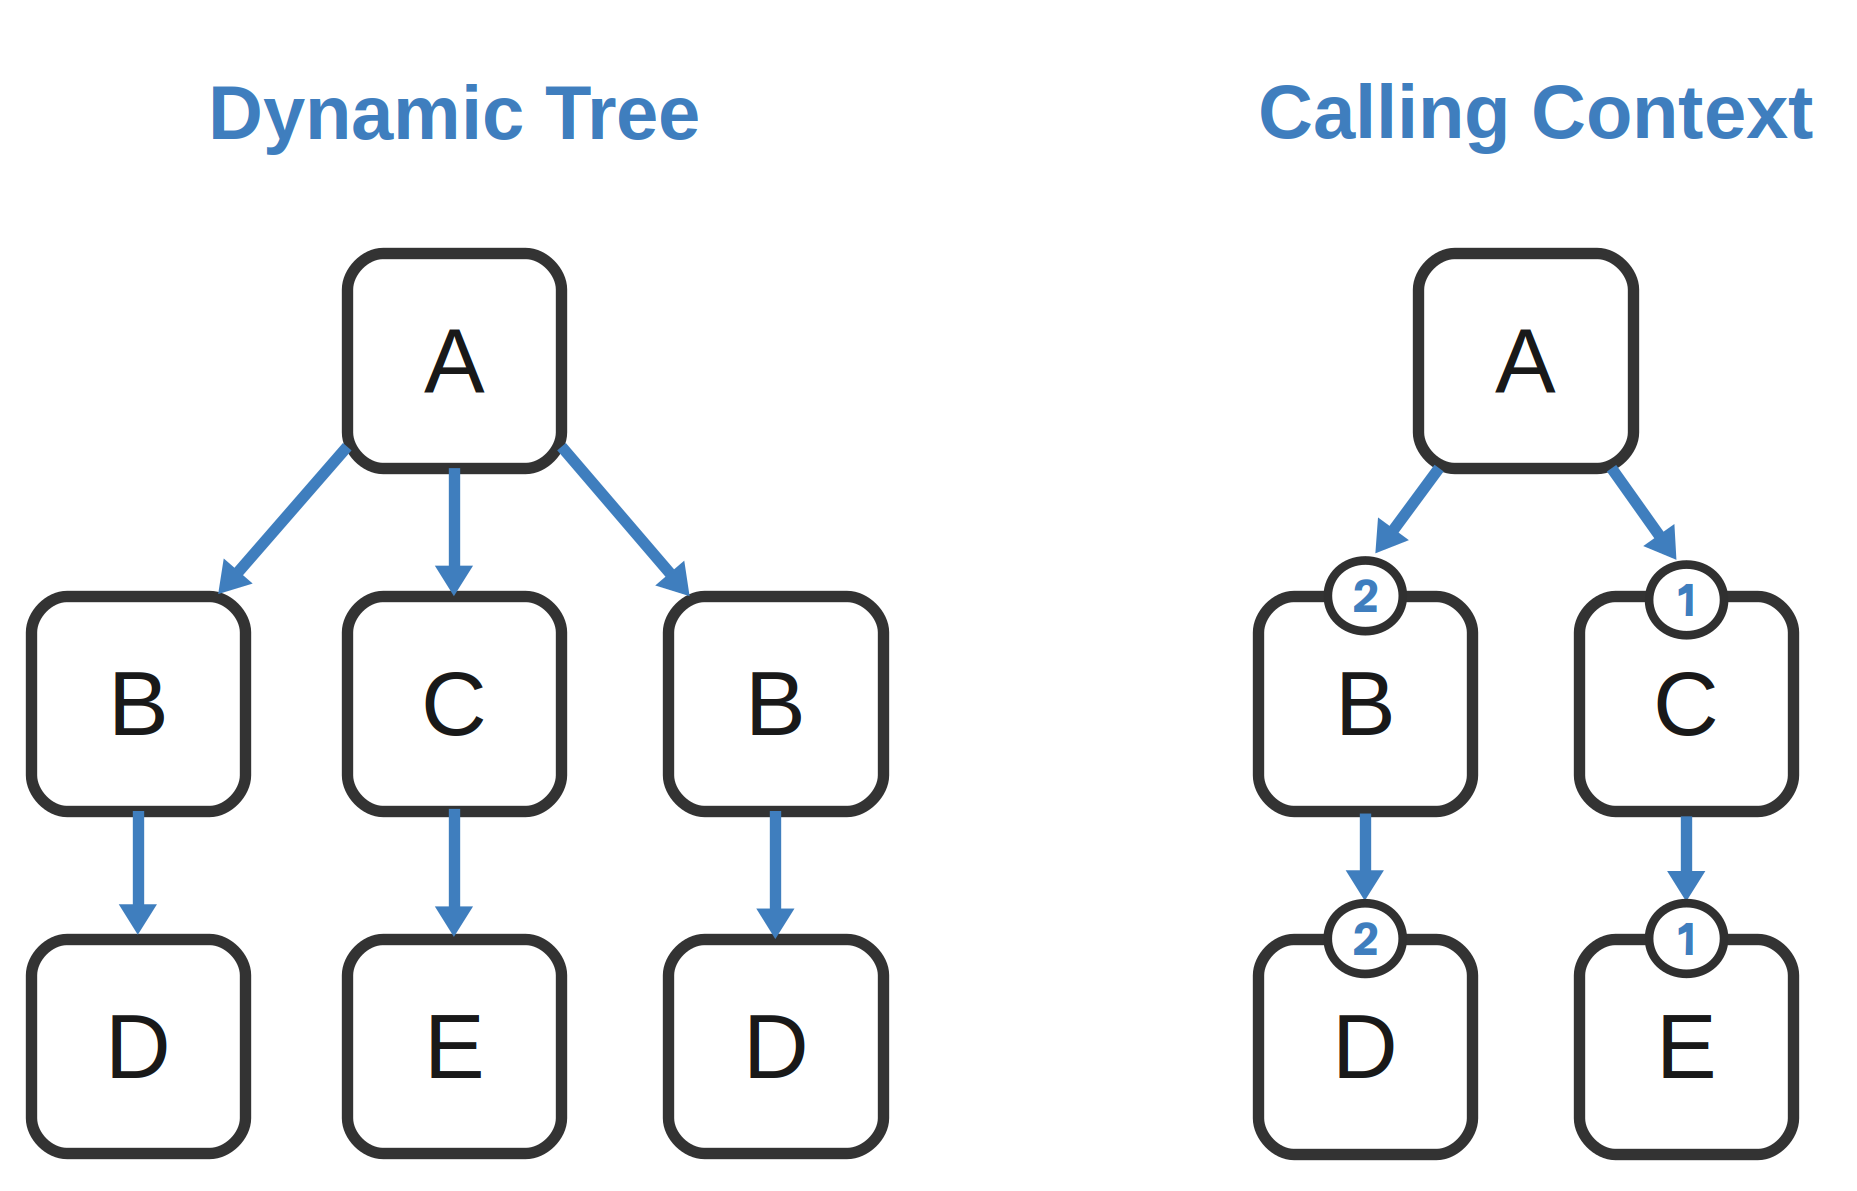
\includegraphics[width=0.40\textwidth]{figures/dynamic-calling.png}
        \caption{Dynamic Call Graph vs Enhanced Calling Context Tree }
        \label{fig:ecct_dt}
    \end{figure}
    The metrics recorded inside the tree are described in the subsection Performance Metrics.
    
\textit{Performance Metrics}\\
    In virtue of generating a tree through a tracing approach, it is possible to record runtime information of the system \cite{francis1}.
    They are recorded using the lttng feature add-context, and this gives the possibility to add performance counters in the tracing session.\\
    Example: perf:cache-misses, perf:major-faults, perf:branch-load-misses\\
    This technique was explored in the work of \cite{doray_thesis} and \cite{olsa}.
    Although we took several metrics in consideration, we summarizes three metrics before introduce the clustering mechanism.\\
    
%\textbf{cache-misses}\\ 
%       When a program accesses a memory location that is not in the cache, it is called a cache miss. Since the processor has to wait for the data to be fetched from the next cache level or from main memory before it can continue to execute, cache misses directly influence the performance of the application \cite{washington}.
%       The concept of cache miss ratio, is the ratio of memory accesses that cause a cache miss. From the miss ratio you can usually tell whether cache misses may be a performance problem in an application.
      
%\textbf{page-faults}\\
%       A page fault is the sequence of events occurring when a program attempts to access data (or code) that is in its address space, but is not currently located in the system's RAM. The operating system must handle page faults by somehow making the accessed data memory resident, allowing the program to continue operation as if the page fault had never occurred\cite{redhat}.
      
%\textbf{cpu instructions}\\ 
%       This metric is the measurement of the instructions related to arithmetic, logical and shift operations on values in registers. 
    
    
\subsection{Data Structure Construction}
    The construction of the ECCT involves the reading of the tracing in order and simultaneously building the nodes as soon as the data is coming. It is necessary to delimit the boundaries of the nodes in the tree. Therefore, to set events as starting and end points of the nodes. Depending on the case, the construction of the tree depending on the case might be easy to be done using a ECT, instead of ECCT.\\
    Consequently, it is necessary to demultiplex the events on the trace. To do so, the trace must provide a way to identify the start and end points of each execution. 
    For this process there are two approaches:\\
    First, use existing events of the Linux kernel. As an example, the syscall\_exit\_accept event (generated when a connection is accepted on a socket) and the syscall\_entry\_shutdown event (generated when a connection is closed) correctly delimit requests received by an Apache server. \\
    Second, is to use LTTng-UST probes, statically inserted in the source code. Different probe types can be used to delimit different execution types. In that way, the delimitation of the nodes can be done.
    An advantage the first approach is to use existing events and thus, no access to the source code is required. The advantages of the second is that no kernel knowledge is required to use this process.
    
    The Figure \ref{fig:ecct_build}, demonstrates the mechanism used to create the ECCT from the tracing file.
    
\begin{figure}[h]
      \centering
        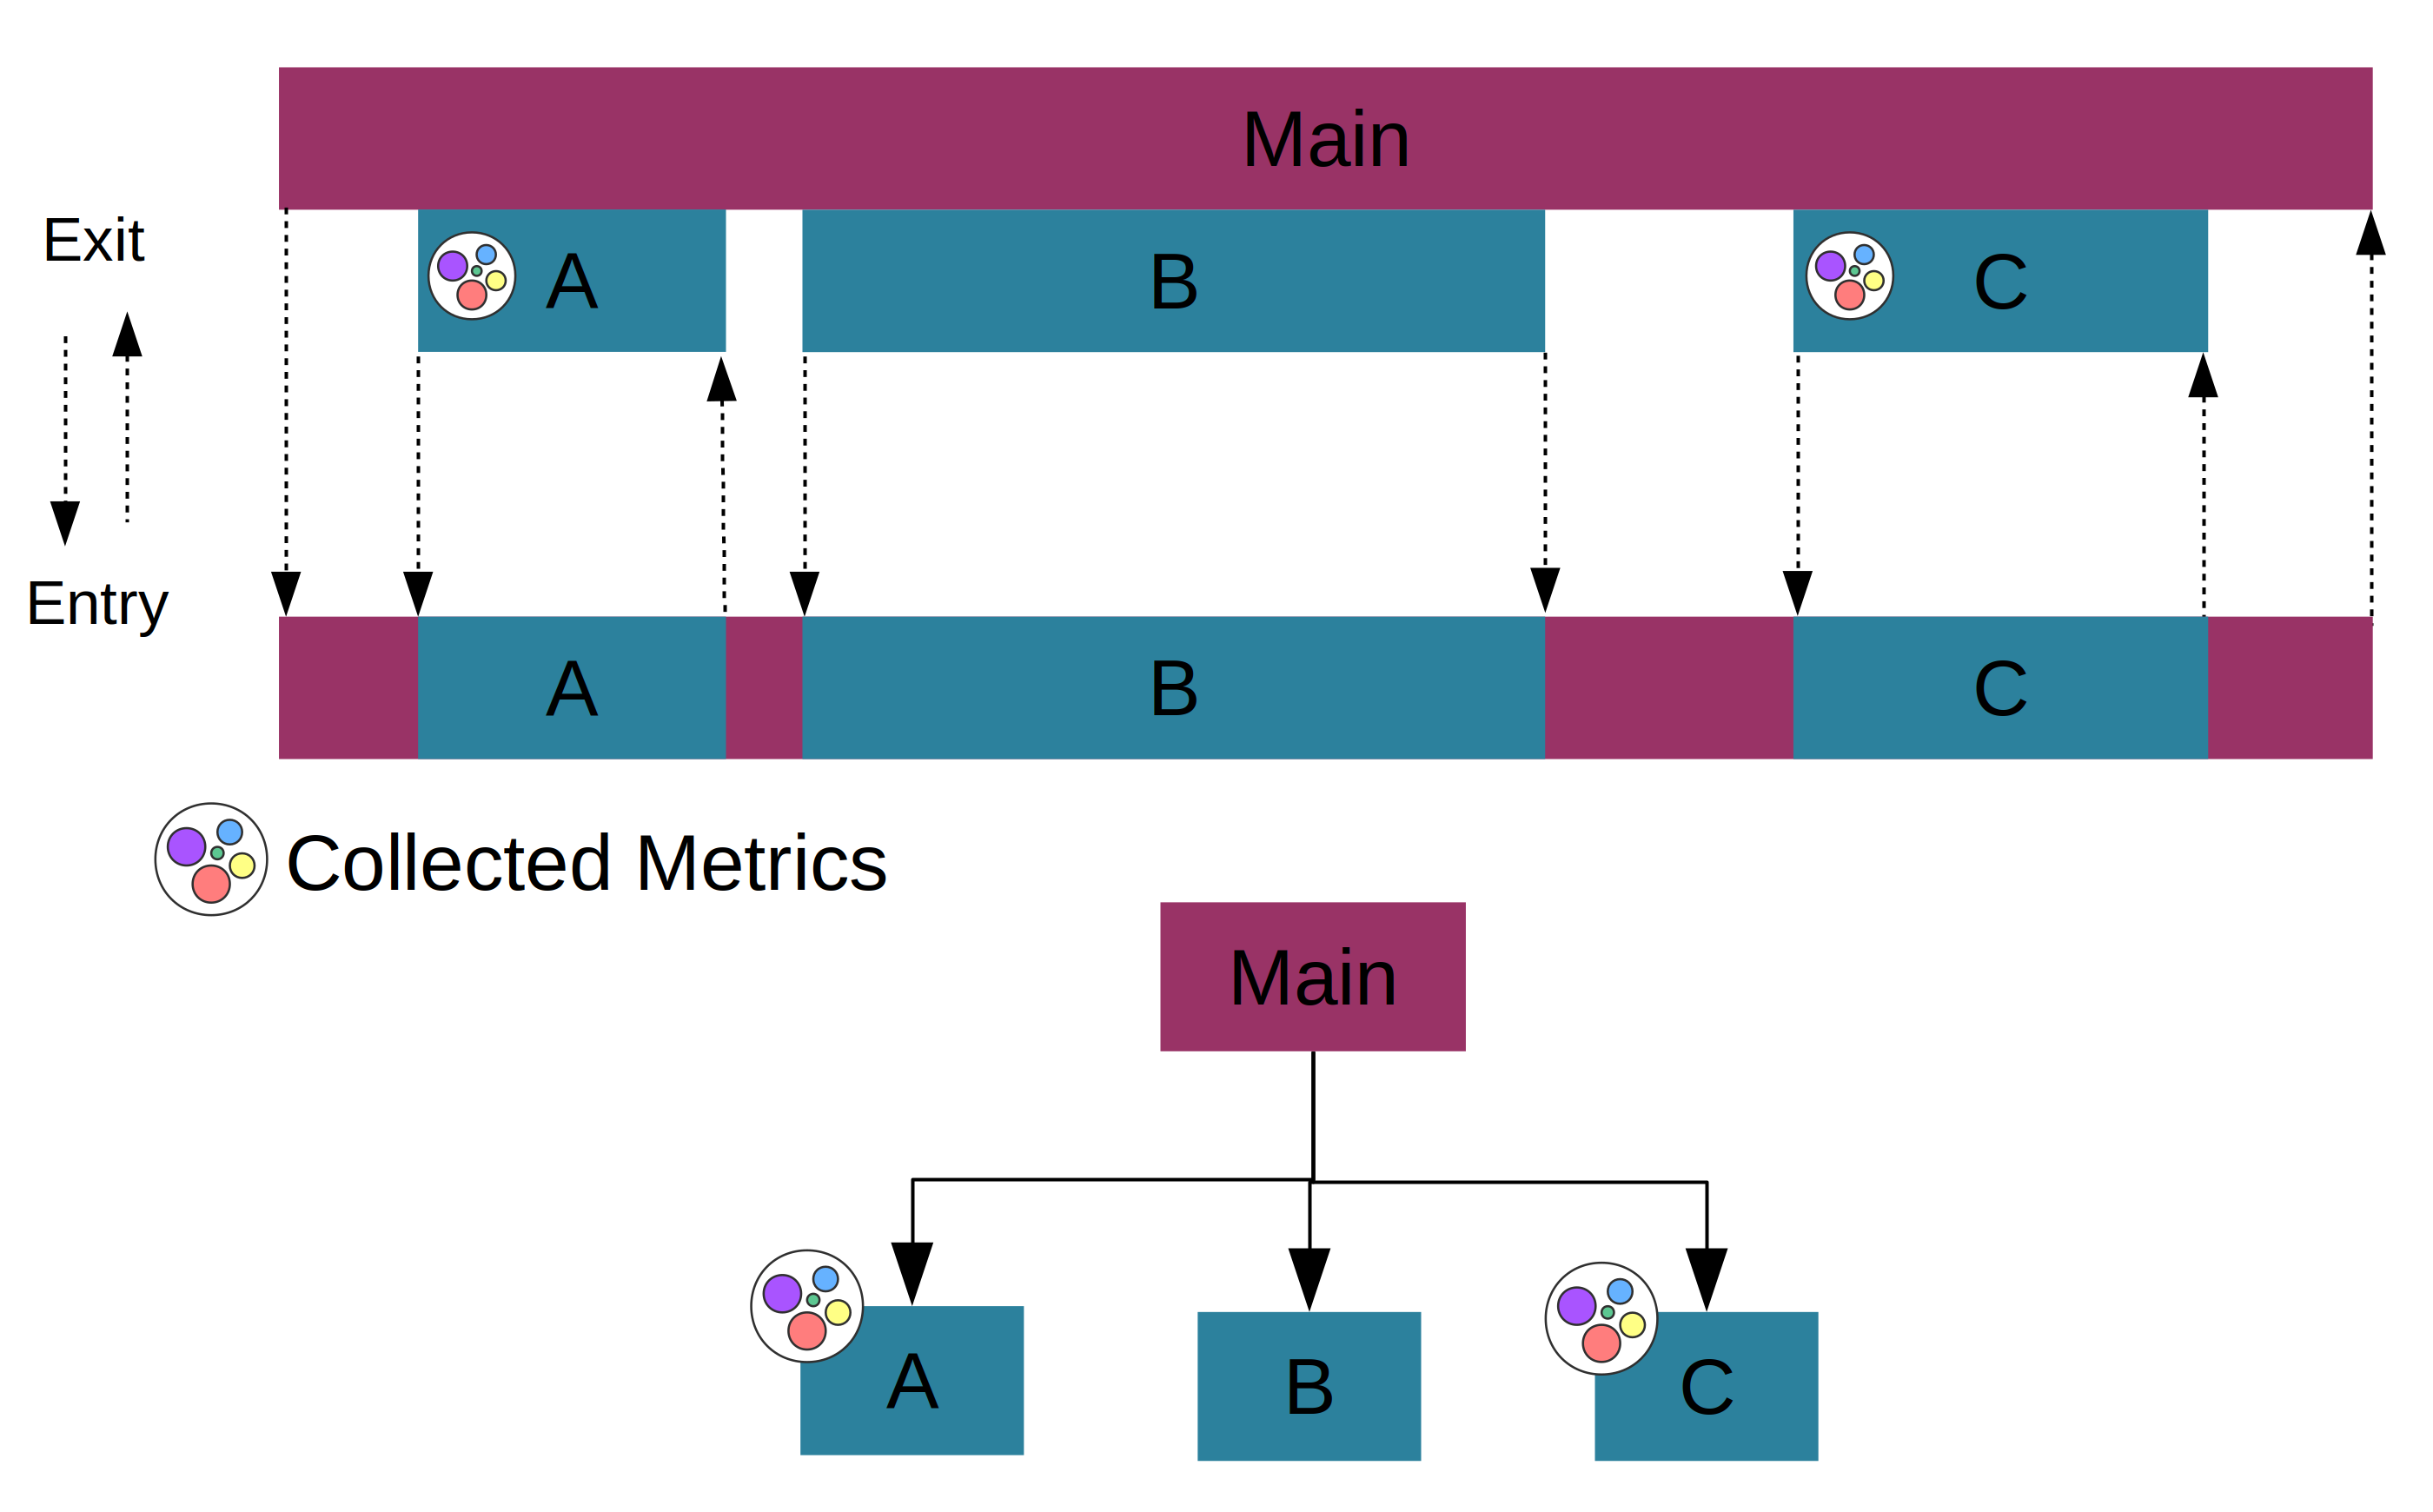
\includegraphics[width=0.50\textwidth]{figures/ecct.png}
        \caption{Enhanced Calling Context}
        \label{fig:ecct_build}
    \end{figure}
    
    After the construction of the tree the clustering mechanisms, described below, can be applied.\\
  
\subsection{Clustering}
\label{sec:clustering}
On this part we outline the clustering techniques used for the metrics grouping, the heuristic to do an automated classification mechanisms and finally the association rule used to find the metric which impacted on the performance of the executions.\\

% \textbf{Clustering techniques}
% \textit{ Supervised and non-supervised machine learn methods}\\
%     Supervised learning is the machine learning task of inferring a function from labeled training data. The training data consist of a set of training examples. In supervised learning, each example is a pair consisting of an input object (typically a vector) and a desired output value (also called the supervisory signal). A supervised learning algorithm analyzes the training data and produces an inferred function, which can be used for mapping new examples. 
    
%     Unsupervised machine learning is the machine learning task of inferring a function to describe hidden structure from "unlabeled" data (a classification or categorization is not included in the observations). Since the examples given to the learner are unlabeled, there is no objective evaluation of the accuracy of the structure that is output by the relevant algorithm—which is one way of distinguishing unsupervised learning from supervised learning and reinforcement learning.
    
\textit{Support Vector Machines}\\
In machine learning, support vector machines are supervised learning models with associated learning algorithms that analyze data used for classification and regression analysis. Given a set of training examples, each marked as belonging to one or the other of two categories, an SVM training algorithm builds a model that assigns new examples to one category or the other, making it a non-probabilistic binary linear classifier. 
Besides teaching the model, the restriction is another drawback of using SVMs. The major drawback of this model is the division in two groups, so relevant information could be lost and no further comparison technique could be applied later.

    
% \textit{Mean Swift}\\
%     MeanShift clustering aims to discover blobs in a smooth density of samples. It is a centroid based algorithm, which works by updating candidates for centroids to be the mean of the points within a given region. These candidates are then filtered in a post-processing stage to eliminate near-duplicates to form the final set of centroids.
%     Given a candidate centroid x i for iteration t, the candidate is updated according to the following equation:
    
%     %x_i^{t+1} = x_i^t + m(x_i^t)
    
%     Where N(xi) is the neighborhood of samples within a given distance around xi and m is the mean shift vector that is computed for each centroid that points towards a region of the maximum increase in the density of points. This is computed using the following equation, effectively updating a centroid to be the mean of the samples within its neighborhood:
%     %m(x_i) = \frac{\sum_{x_j \in N(x_i)}K(x_j - x_i)x_j}{\sum_{x_j \in N(x_i)}K(x_j - x_i)}
    
%     The algorithm automatically sets the number of clusters, instead of relying on a parameter bandwidth, which dictates the size of the region to search through. This parameter can be set manually, but can be estimated using the provided estimate bandwidth function, which is called if the bandwidth is not set.
%     The algorithm is not highly scalable, as it requires multiple nearest neighbor searches during the execution of the algorithm. The algorithm is guaranteed to converge, however the algorithm will stop iterating when the change in centroids is small \cite{mean_swift}.

\textit{Percentage classification}\\
The percentage classification was done by comparing the metrics and separate them by a percentage threshold, which is the mean of the group. The percentage classification is interesting considering sometimes that the distribution is not so spaced to create clusters. The naive classification will draw a group even when they are too close and would be in just one group for other clustering techniques.
    
\textit{K-means}\\
K-means is a simple unsupervised machine learning algorithm that groups a dataset into a user-specified number (k) of clusters. The algorithm is somewhat naive it clusters the data into k clusters, even if k is not the right number of clusters to use. Therefore, when using k-means clustering, users need some way to determine whether they are using the right number of clusters.
Since, the number of groups must be known before applying the k-means, another technique needs to be applied in order to find the appropriate number of groups (k). 
    
    
\textit{Comparing Models}\\
Comparing the three techniques described above, the conclusions were. First, the SVM model was able to delimit the difference between the slow executions and fast executions. However, the delimitation is in just two groups. \\
The second mechanism, Percentage classification, is a unsupervised mechanism and leads to segregation of data even if they are homogeneously distributed among the dataset. \\
Finally the k-means algorithm is efficient but requires the number of groups to be used in the classification process. Comparing the models we developed the technique to use an heuristic classification to make the clustering process automatic.
    
    
\textit{Auto Clustering}\\
Considering the models shown above, we chose to develop a non-supervised method, called auto clustering. The possibility to use an automated approach is more interesting for us in comparison with a non-automated methods, mainly because we aim not to use the data to train the model. Therefore we implemented a version of comparative k-means using the SSE (sum of square errors) variability information, plus an heuristic evaluation. This technique can be used for an arbitrary dimension of since the amount of difference, SSE (sum of squared error), can be calculated on those cases \cite{multi_dimentionals_sse}.
    
\subsection{\textbf{Automatic Clustering through heuristic Evaluation}}

    \textit{Elbow method}\\
    One method to quantitatively measure the number of clusters is the elbow method. This method compares the sum of squared errors (SSE) considering several numbers of groups from the classification used. 
    The elbow method gives the possibility to use the SSE to find the elbow value, which can be defined as a value which the SSE changes its behaviour abruptly. In our cases, the elbow value is when the SSE stop decreasing substantially.
    
    However, the elbow method does not guarantee a perfect match in cases which the data is well distributed. Instead, the analysis of the SSE can give a smooth curve and the best value for number of groups is not precisely defined. In cases like this, we developed another clustering based on the mean distance of the data.
    %try a different method for determining the optimal k, such as computing silhouette scores, or we might reevaluate whether clustering is the right thing to do on our data.
    
    \textit{Heuristic Evaluation}\\
    To compare the SSE values, we needed also to do an heuristic function which compares the different values of the SSE to compute the Elbow. 
    Therefore, we use this approach to compare several runs of classifications and extract the one with less squared errors. The used heuristic is to take as optimal group the biggest gap on an array of SSE values. 
    
    The Figure \ref{fig:sse}, shows an illustration of the SSE and the elbow value. The elbow value is the number that marks the change on the path of the function, in the example is number of groups 2.
    
    \begin{figure}[h]
      \centering
        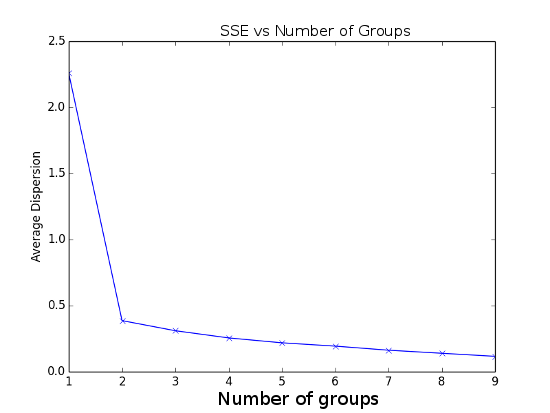
\includegraphics[width=0.50\textwidth]{figures/SSE.png}
        \caption{Elbow method: SSE Comparison}
        \label{fig:sse}
    \end{figure}


\subsection{\textbf{Association among the Groups}}
\label{sec:association}
The clustering of metrics is just a part of the approach, since a rule of groups need to be applied to find the specific cause for the discrepancy on the executions. To solve this problem and find the cause of the difference, after the grouping mechanism we applied a set association rule. Therefore, using a set exclusion, we can find the metric that is responsible for the elapsed time.
The association rule is illustrated on the Figure \ref{fig:association}, which describes a metric X and the elapsed time comparison. The grouping on the Metric x divides the data in two groups and those groups are the intrinsic related to the elapsed time group. \\
The association rule can be applied in an arbitrary classification algorithm with several different dimensions, so the association can be defined as a heuristic to find root cause problems using grouping or clustering algorithms.

A matrix of groups correlation can be done to better understand the relation among the groups.


    % \begin{figure}[h]
    %   \centering
    %     \includegraphics[width=0.50\textwidth]{figures/association.png}
    %     \caption{Association of groups through Apriori algorithm}
    %     \label{fig:association}
    % \end{figure}
    
\begin{table}[h]
\centering
\begin{tabular}{cccc}
                      & A                         & B                        & C     \\ \hline
                      &                           &                          &       \\ 
A                     & X                         & 75\%                     & 100\% \\ \hline
                      &                           &                          &       \\ 
B                     & 75\%                      & X                        & 65\%  \\ \hline
                      &                           &                          &       \\
\multicolumn{1}{l}{C} & \multicolumn{1}{l}{100\%} & \multicolumn{1}{l}{65\%} & X     \\ \hline
\end{tabular}
\vspace{10pt}
\caption{Association of groups through Apriori algorithm}
\label{fig:association}
\end{table}

\subsection{\textbf{Accuracy of the model}}
The association will give the group of metrics that are related with slow and fast runs, however, there is the possibility of false positives and false negatives. The accuracy of the model is related with the size of the groups given, i.e. the all slow executions will be in one group, however the related metric, which explains the reason, is bigger than the associated group.  In summary, if the groups overlap, main metric and slow executions, no false positives of negatives were found, even though the overlap does not mean is responsible for the performance problem, it is only an indication factor. In this matter, statistics is an indicator of underlying causes, which requires some complementary analysis to be confirmed.
    
    
\section{Solution Implementation}
\label{sec:implementaion}
\begin{figure*}[t!]
  \centering
    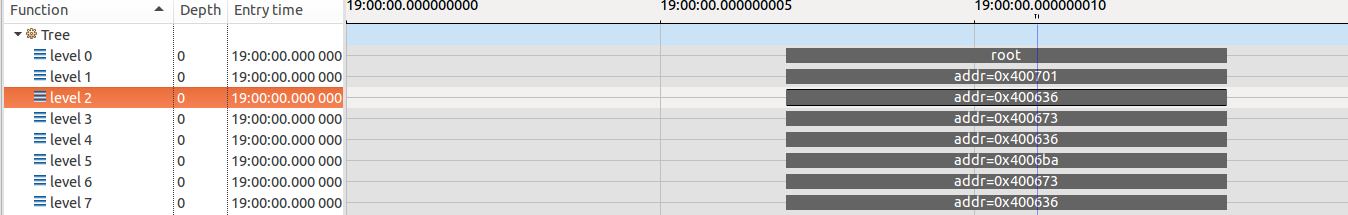
\includegraphics[width=1.0\columnwidth]{figures/cct_view.png}
    \caption{CCT View in TraceCompass }
    \label{fig:cct_view}
    \vspace{-10pt}
\end{figure*}

We describe on this section the implementation of the Calling Context Tree in TraceCompass, the Flame Graph comparison, and the Auto cluster mechanism.

The CCT View is an analysis developed in TraceCompass framework \cite{tracecompass}, which specifically aims to study the CCT and its variations. The module with Auto clustering was included on it. The view displays the calling functions in a graphic view that helps the developer/tester to improve their codes and to compare the traces using the approach described on this work.\\

\textbf{\textit{Tree Construction}}\\
The CCT View builds the tree from the tracing as explained in the section Tree Construction. In summary the tracing is read in order and event entry-exit pairs are grouped in nodes, sub-nodes are defined by pairs of entry-exit inside the above node. The data found, i.e the performance metrics, of the nodes is summarized for the respective node. The tree is build to summarized the redundant nodes, thus, avoiding the build of a Dynamic Call Tree. Figure \ref{fig:cct_view}, shows this feature in the CCT View.\\

\textbf{\textit{Differential Flame Graph}}\\
The CCT View implements a Differential Flame Graph view to compare executions and groups of executions. Usually the Differential Flame Graph compares two executions, but on our implementation it is possible to compare groups of executions. In our implementation the flame graphs are composed of three colors: green (to represent equals amount of time), red (slower executions) and gray (faster executions). 

Figure \ref{fig:flame}, shows a diagram of the RGG Differential Flame Graph, the green color shows the functions which are faster in the main execution, the grey part means they are equal and the red part means that this function is slower with the comparative one. The name, RGG flamegraph brings allusion of this concept in contrast with Brendan Gregg's Red/Blue Flame Graph. 
 
 \begin{figure}[h]
  \centering
    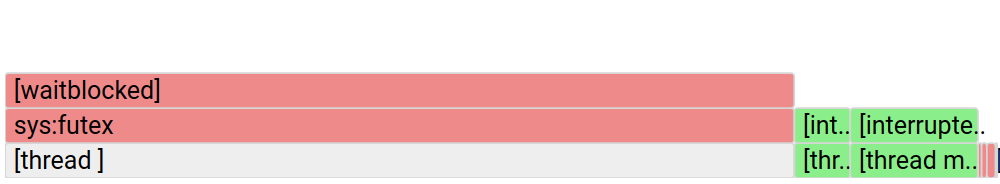
\includegraphics[width=1.0\textwidth]{figures/framegraph.png}
  \caption{RGG Differential Flame Graph Diagram}
  \label{fig:flame}
\end{figure}

\textbf{\textit{Auto cluster}}\\
The Auto cluster feature was implemented on CCTView to help developers execute similar performance cause analysis on tracing. The heuristic evaluation (elbow method) and the clustering techniques (k-means and percentage clustering) were implemented separately, therefore the developer can choose the most suitable one.\\
    
\textbf{\textit{Correlation feature}}\\
Another feature of the CCT View is the possibility to find the correlation matrix of the metrics. 
As the dictum states, \textit{correlation does not imply causation}, which means that correlation by itself cannot be used to infer a causal relationship between the studied variables.
        
    

\label{sec:methodology}
% BENCHMARKS    --------------------------------------------
\section{Benchmarks}
    Considering the several aspects of software performance, here are highlighted some micro-benchmarks which can impact on the performance of the software and could change the performance of software throughout the releases.
    
    \textit{inline}\\
    The inline functions are a C++ enhancement feature to increase the execution time of a program. Functions can be compiled as inline automatically, or can be declared by the programmer as inline functions. The compiler replaces the definition of inline functions at compile time instead of referring function definition at runtime.
    
    However, those functions do not always improve the performance and can deteriorate the performance \cite{inline_site}. To evaluate this claim, we tested this feature with several possibilities: strings, integers, structs, vectors, and classes. Using the inline made the performance better for all of them, except for std::string operations. 
    
    The reason for this difference possibly is related with the dynamic allocation time of strings in C++ as explored by \cite{optc++}. We did several tests with different data structures and objects, and strings seems the more effected by this effect.
    
    After investigation, we came to the conclusion that the root cause of this performance degradation is the influence of cache misses in the operations with string inside inline functions.
    
    Comparing the performance of inline functions and regular functions, the results of the benchmarks are shown in the Figures \ref{fig:notinline} and \ref{fig:inline}. For thousand runs, the average, the mean and the median were high in comparison to use the not inline implementation.
    
    \textit{template functions} \\
     Template functions can decrease the performance of a software.
     According to Jacob B. Matthews, from the university of Chicago, \cite{chicago}, the use of templates decrease efficiency of the C++ compiler's.
     
     
    \textit{virtual functions} \\
     The use of virtual functions has a cost for the dispatching. The work of \cite{dispatch} shows the overhead related with dispatching on C++ codes.
     
    \begin{figure}[h]
      \centering
        % 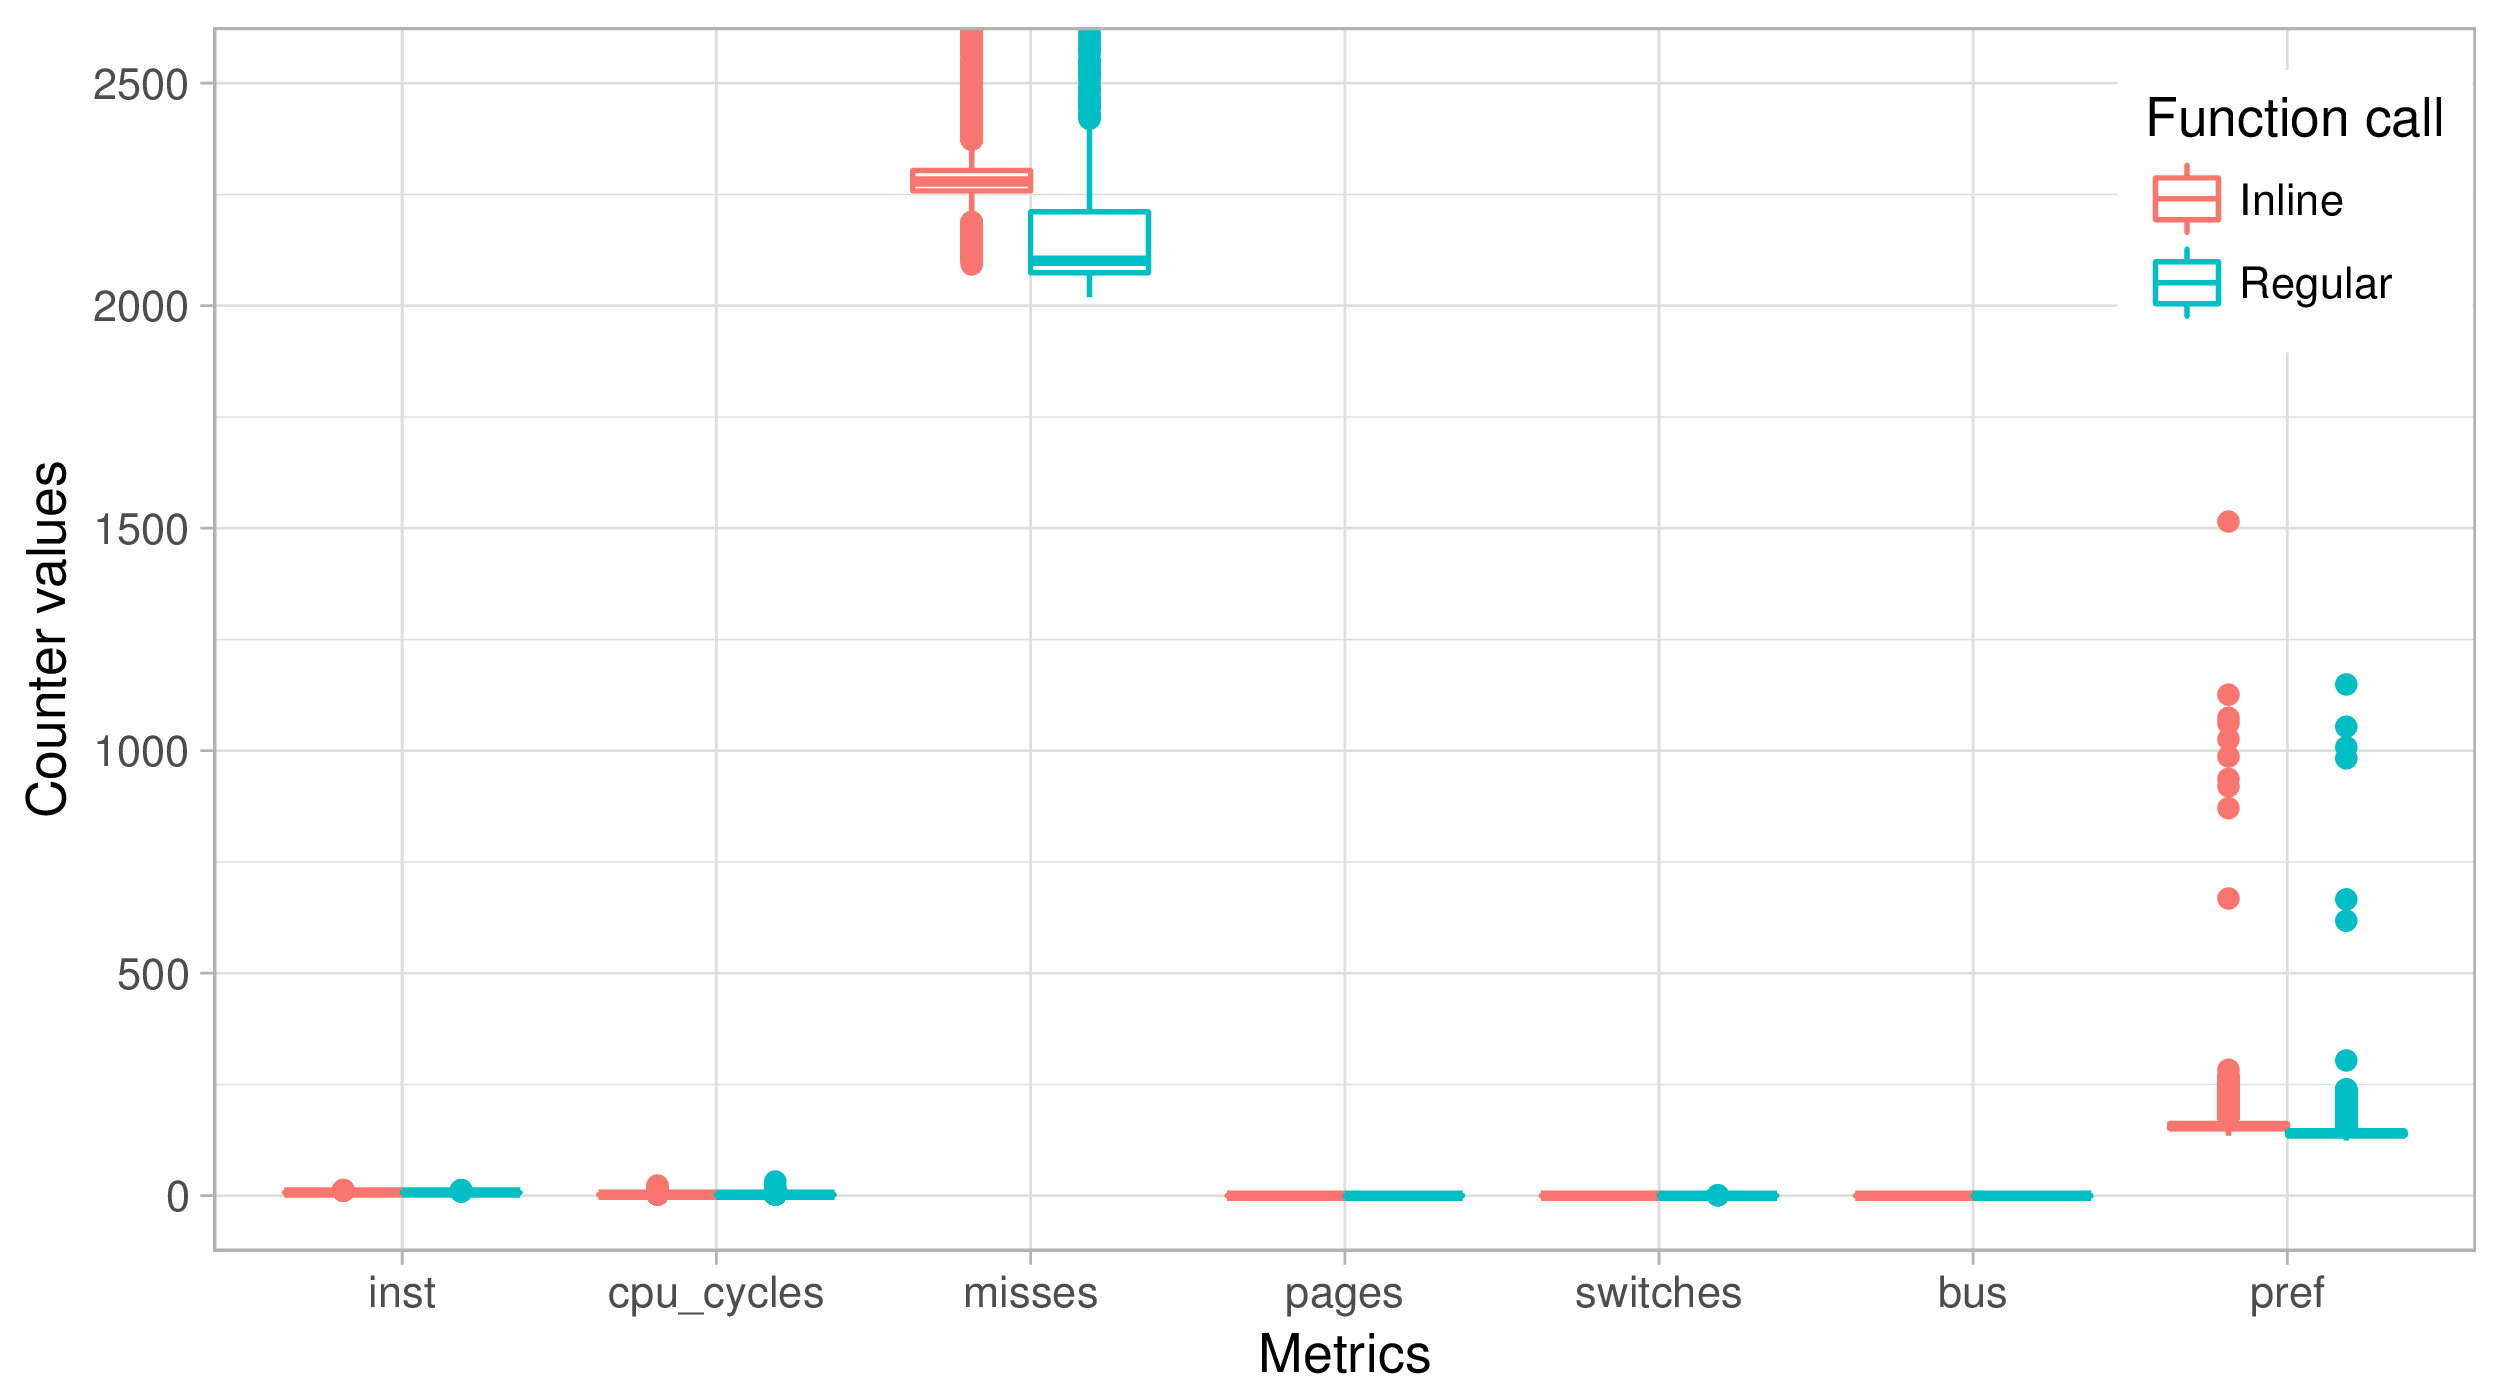
\includegraphics[width=0.47\textwidth]{figures/boxplots-inline-vs-regular.png}
        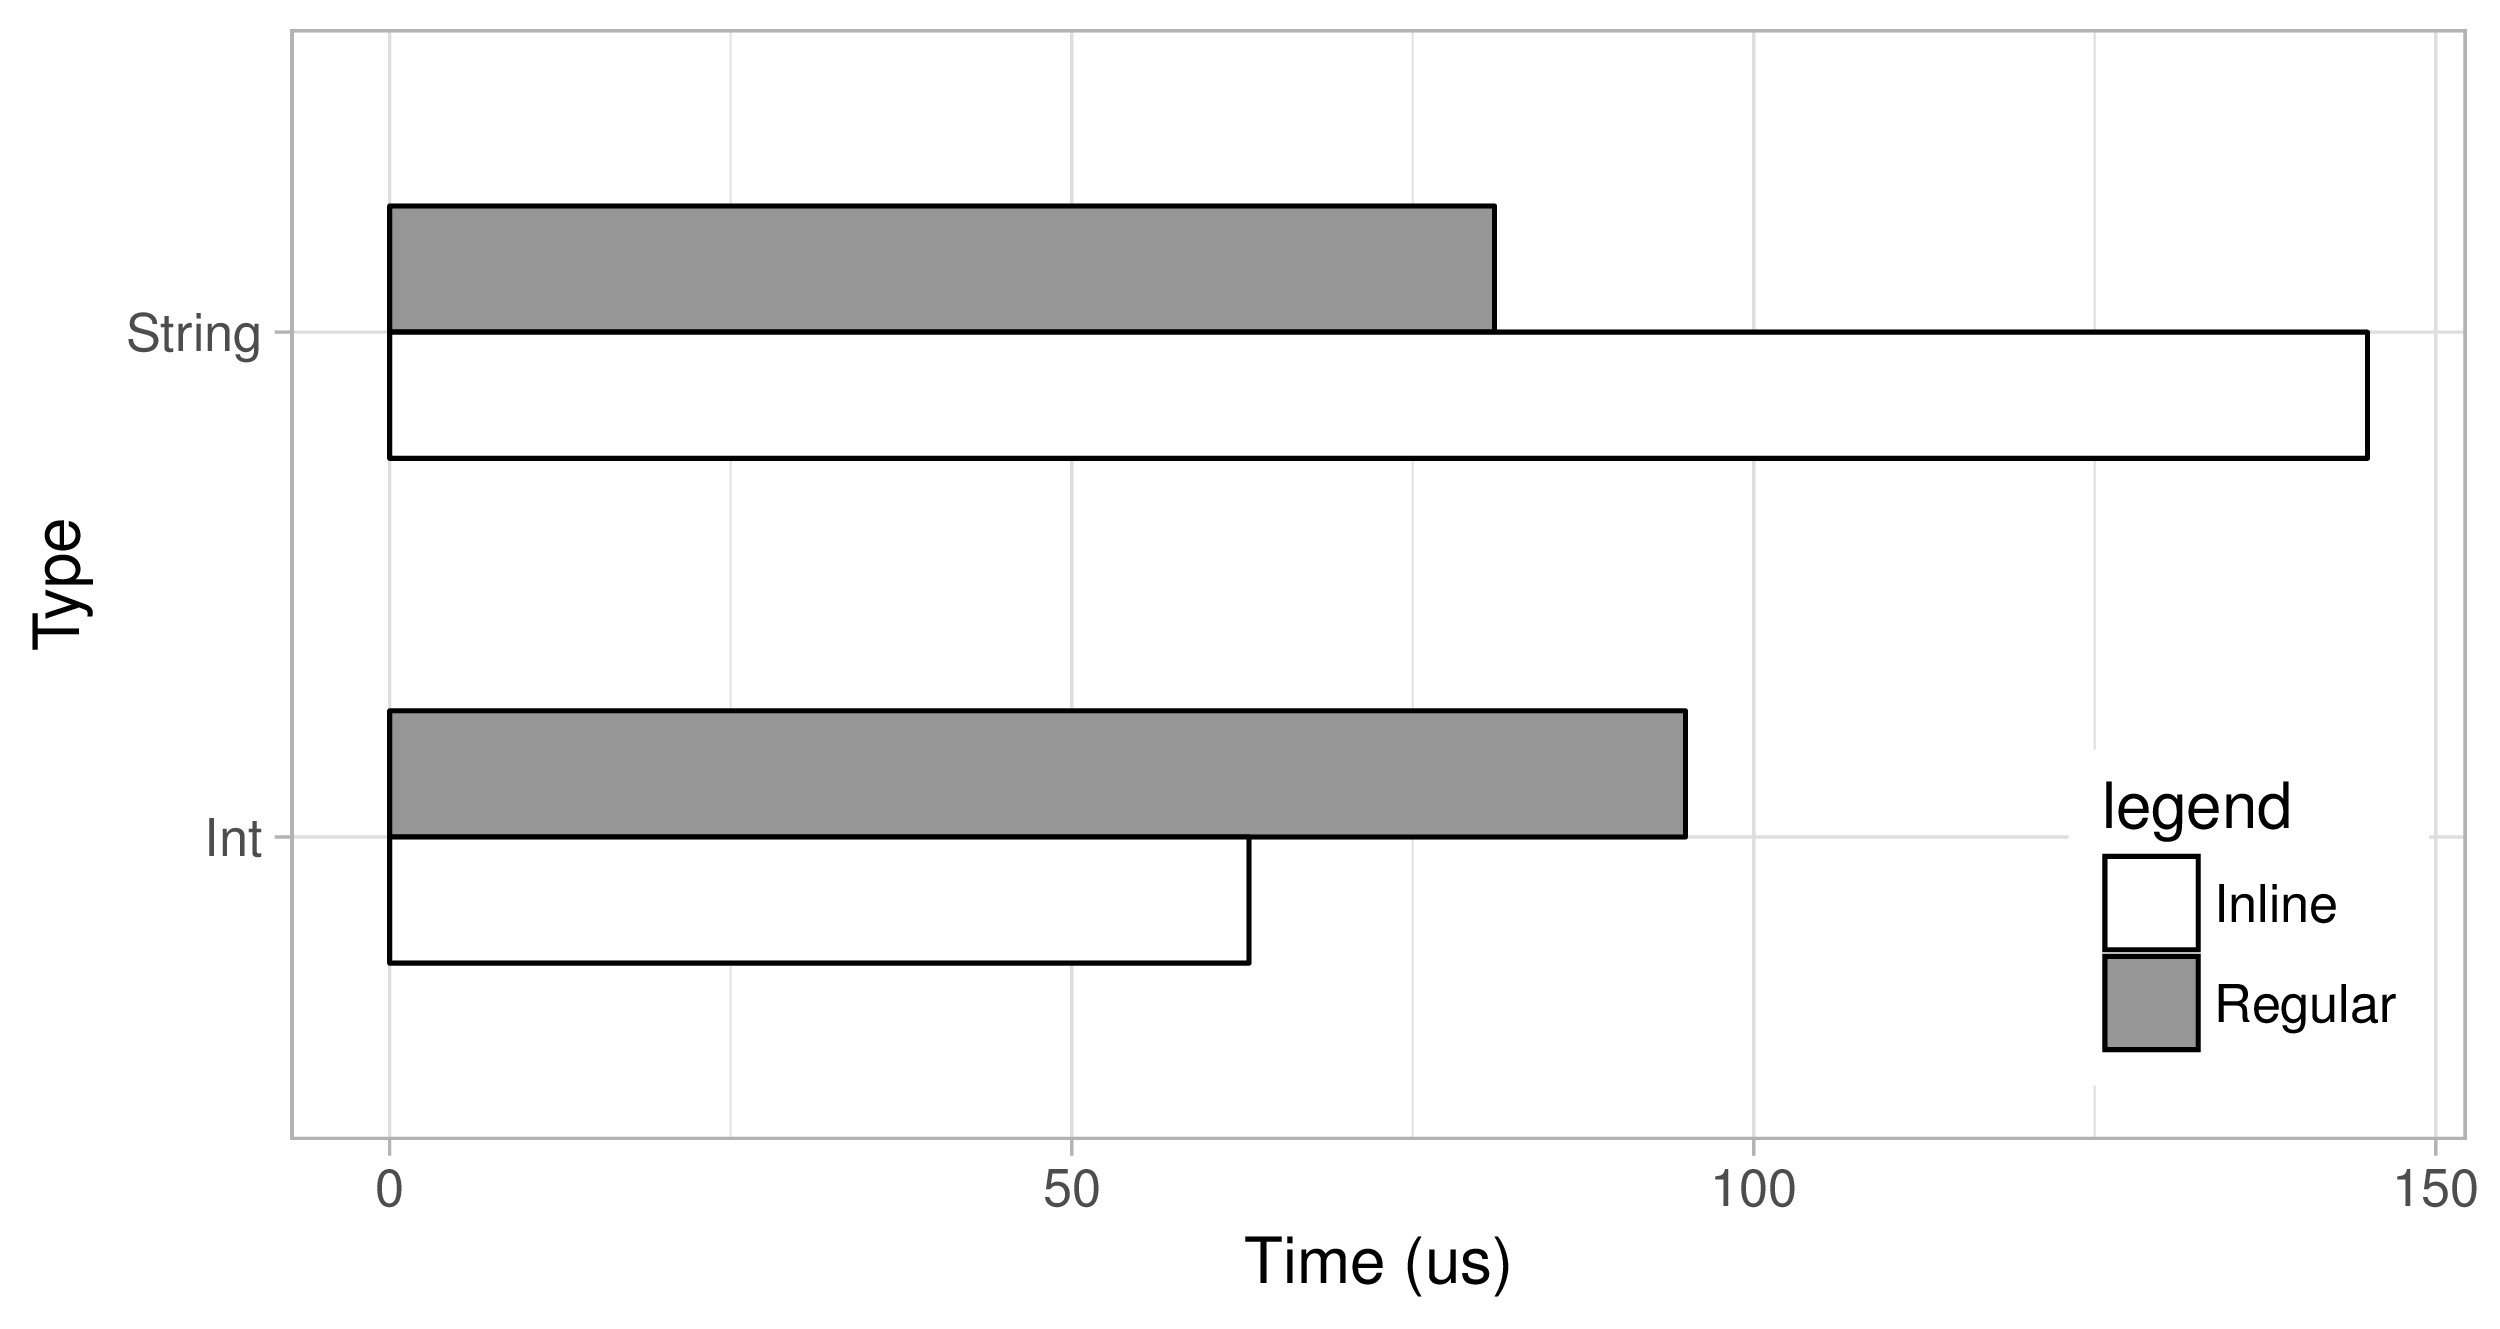
\includegraphics[width=0.6\textwidth]{figures/bar-inline-vs-regular.png}
        \caption{Counter Metrics for Inline and Regular function calls}
        \label{fig:notinline}
    \end{figure}
    
    \begin{figure}[h]
      \centering
        % 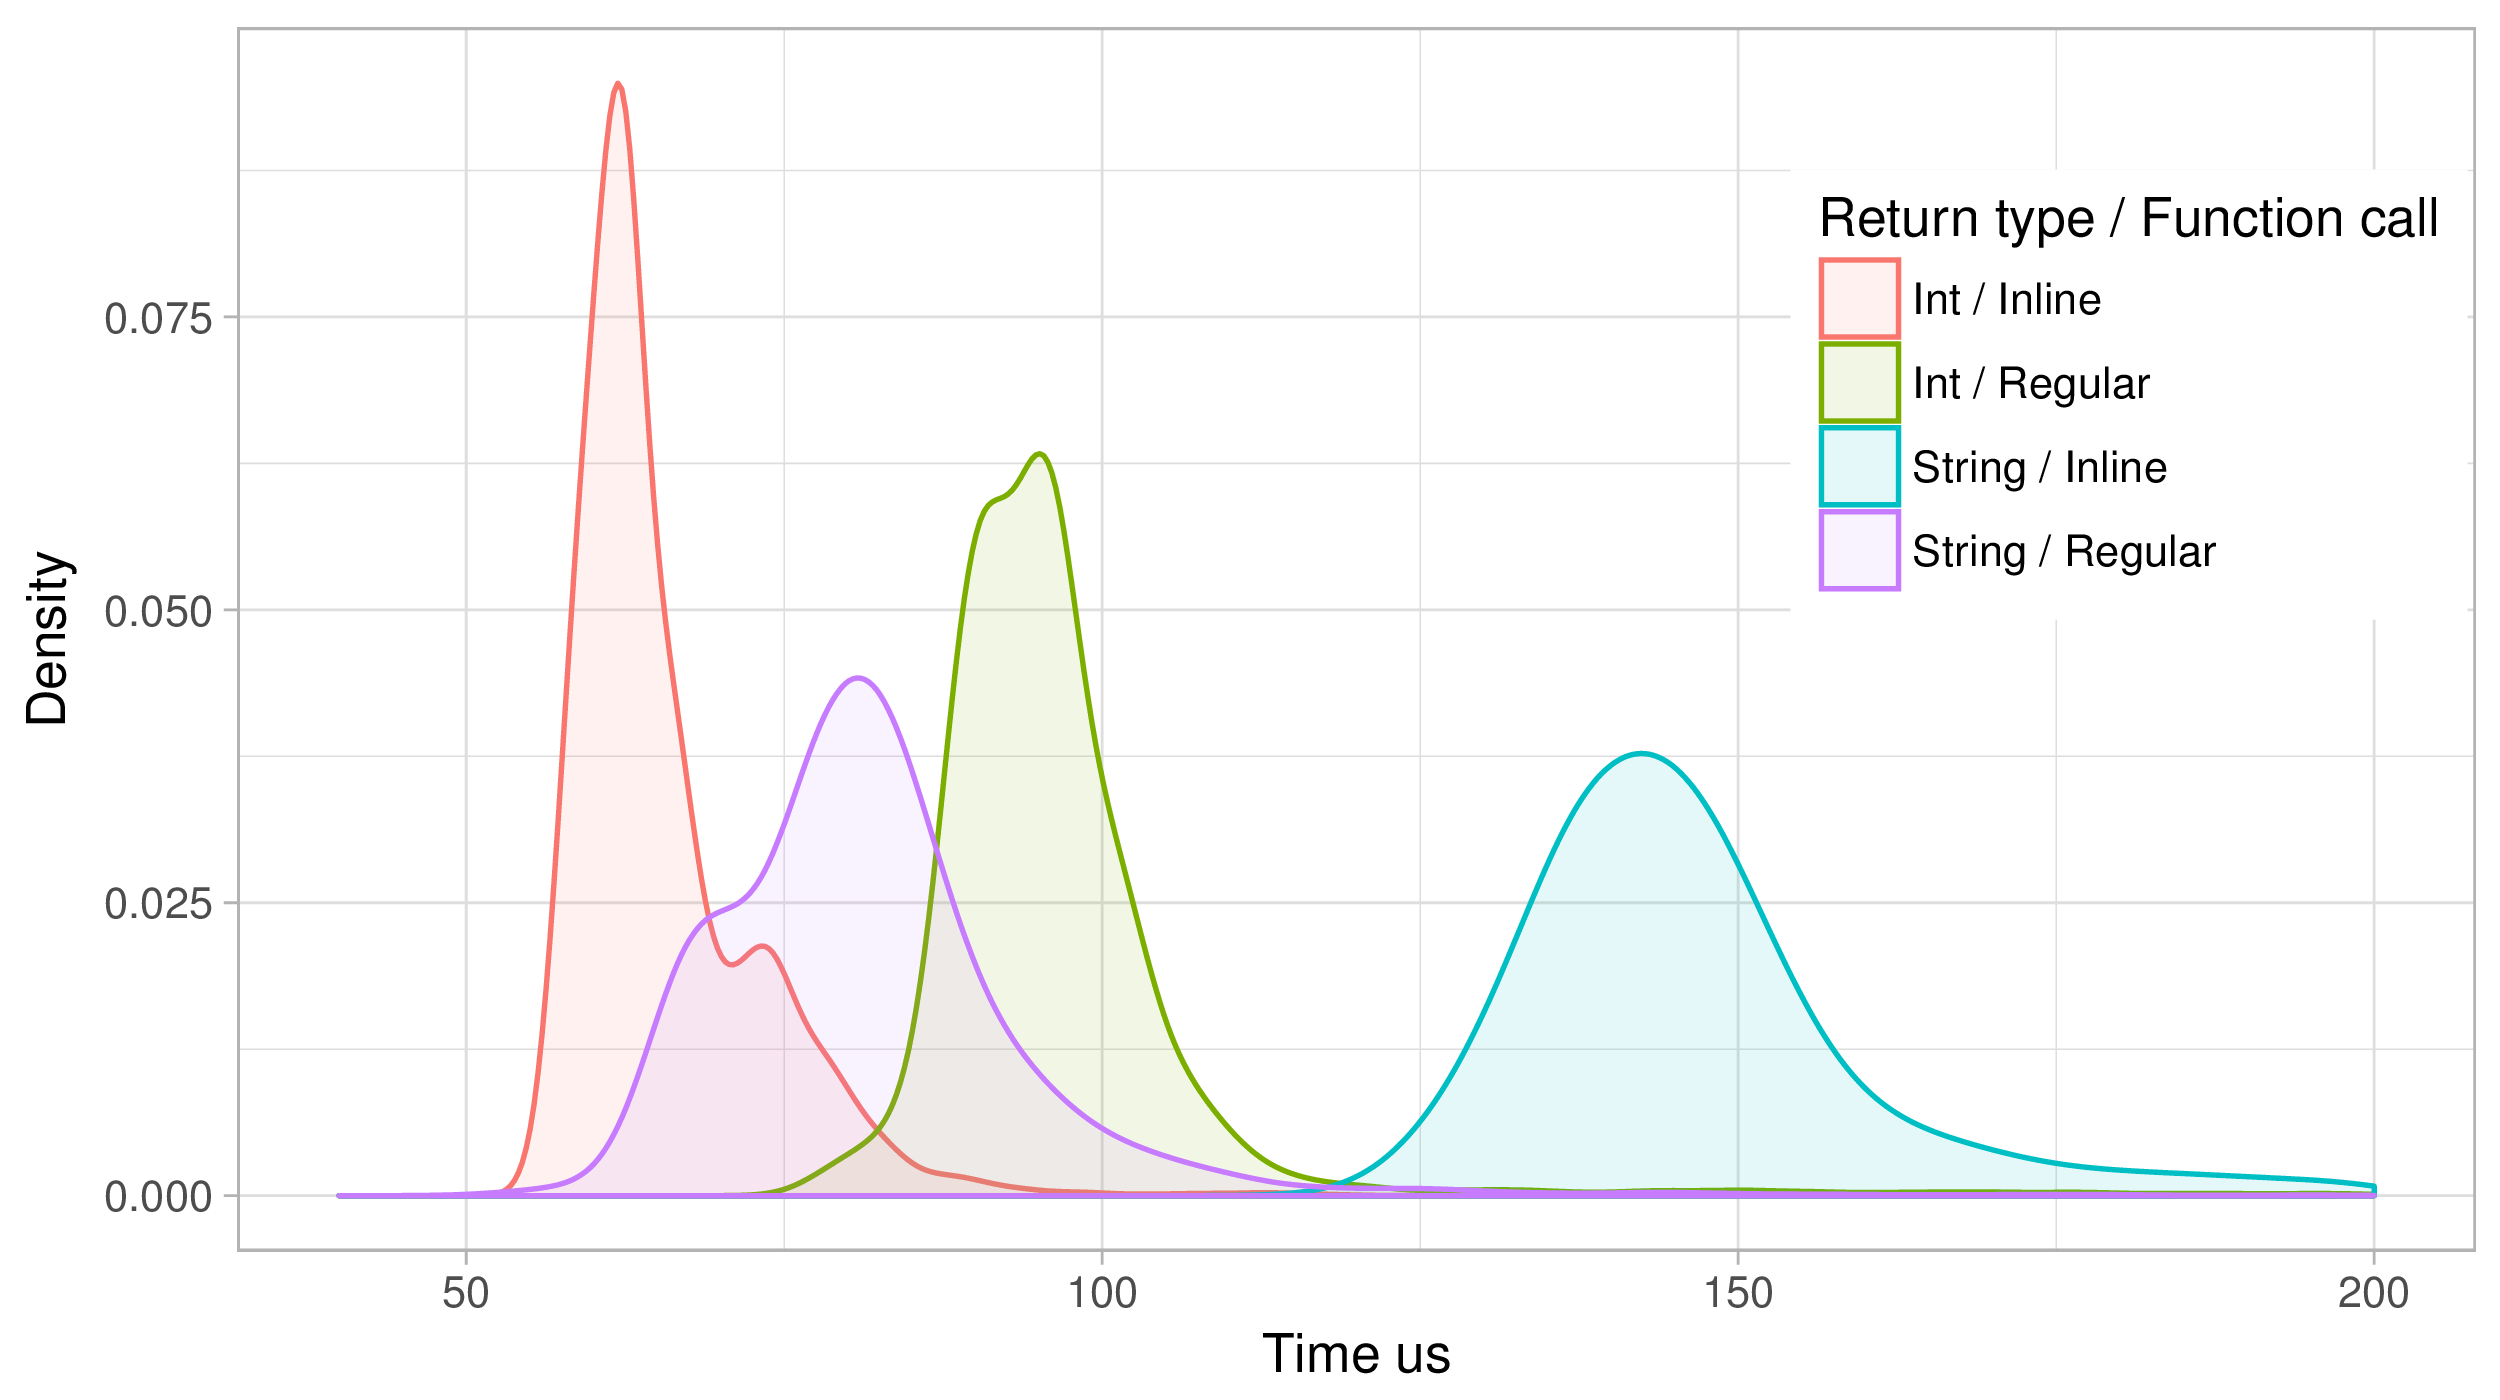
\includegraphics[width=0.47\textwidth]{figures/density-inline-vs-regular.png}
        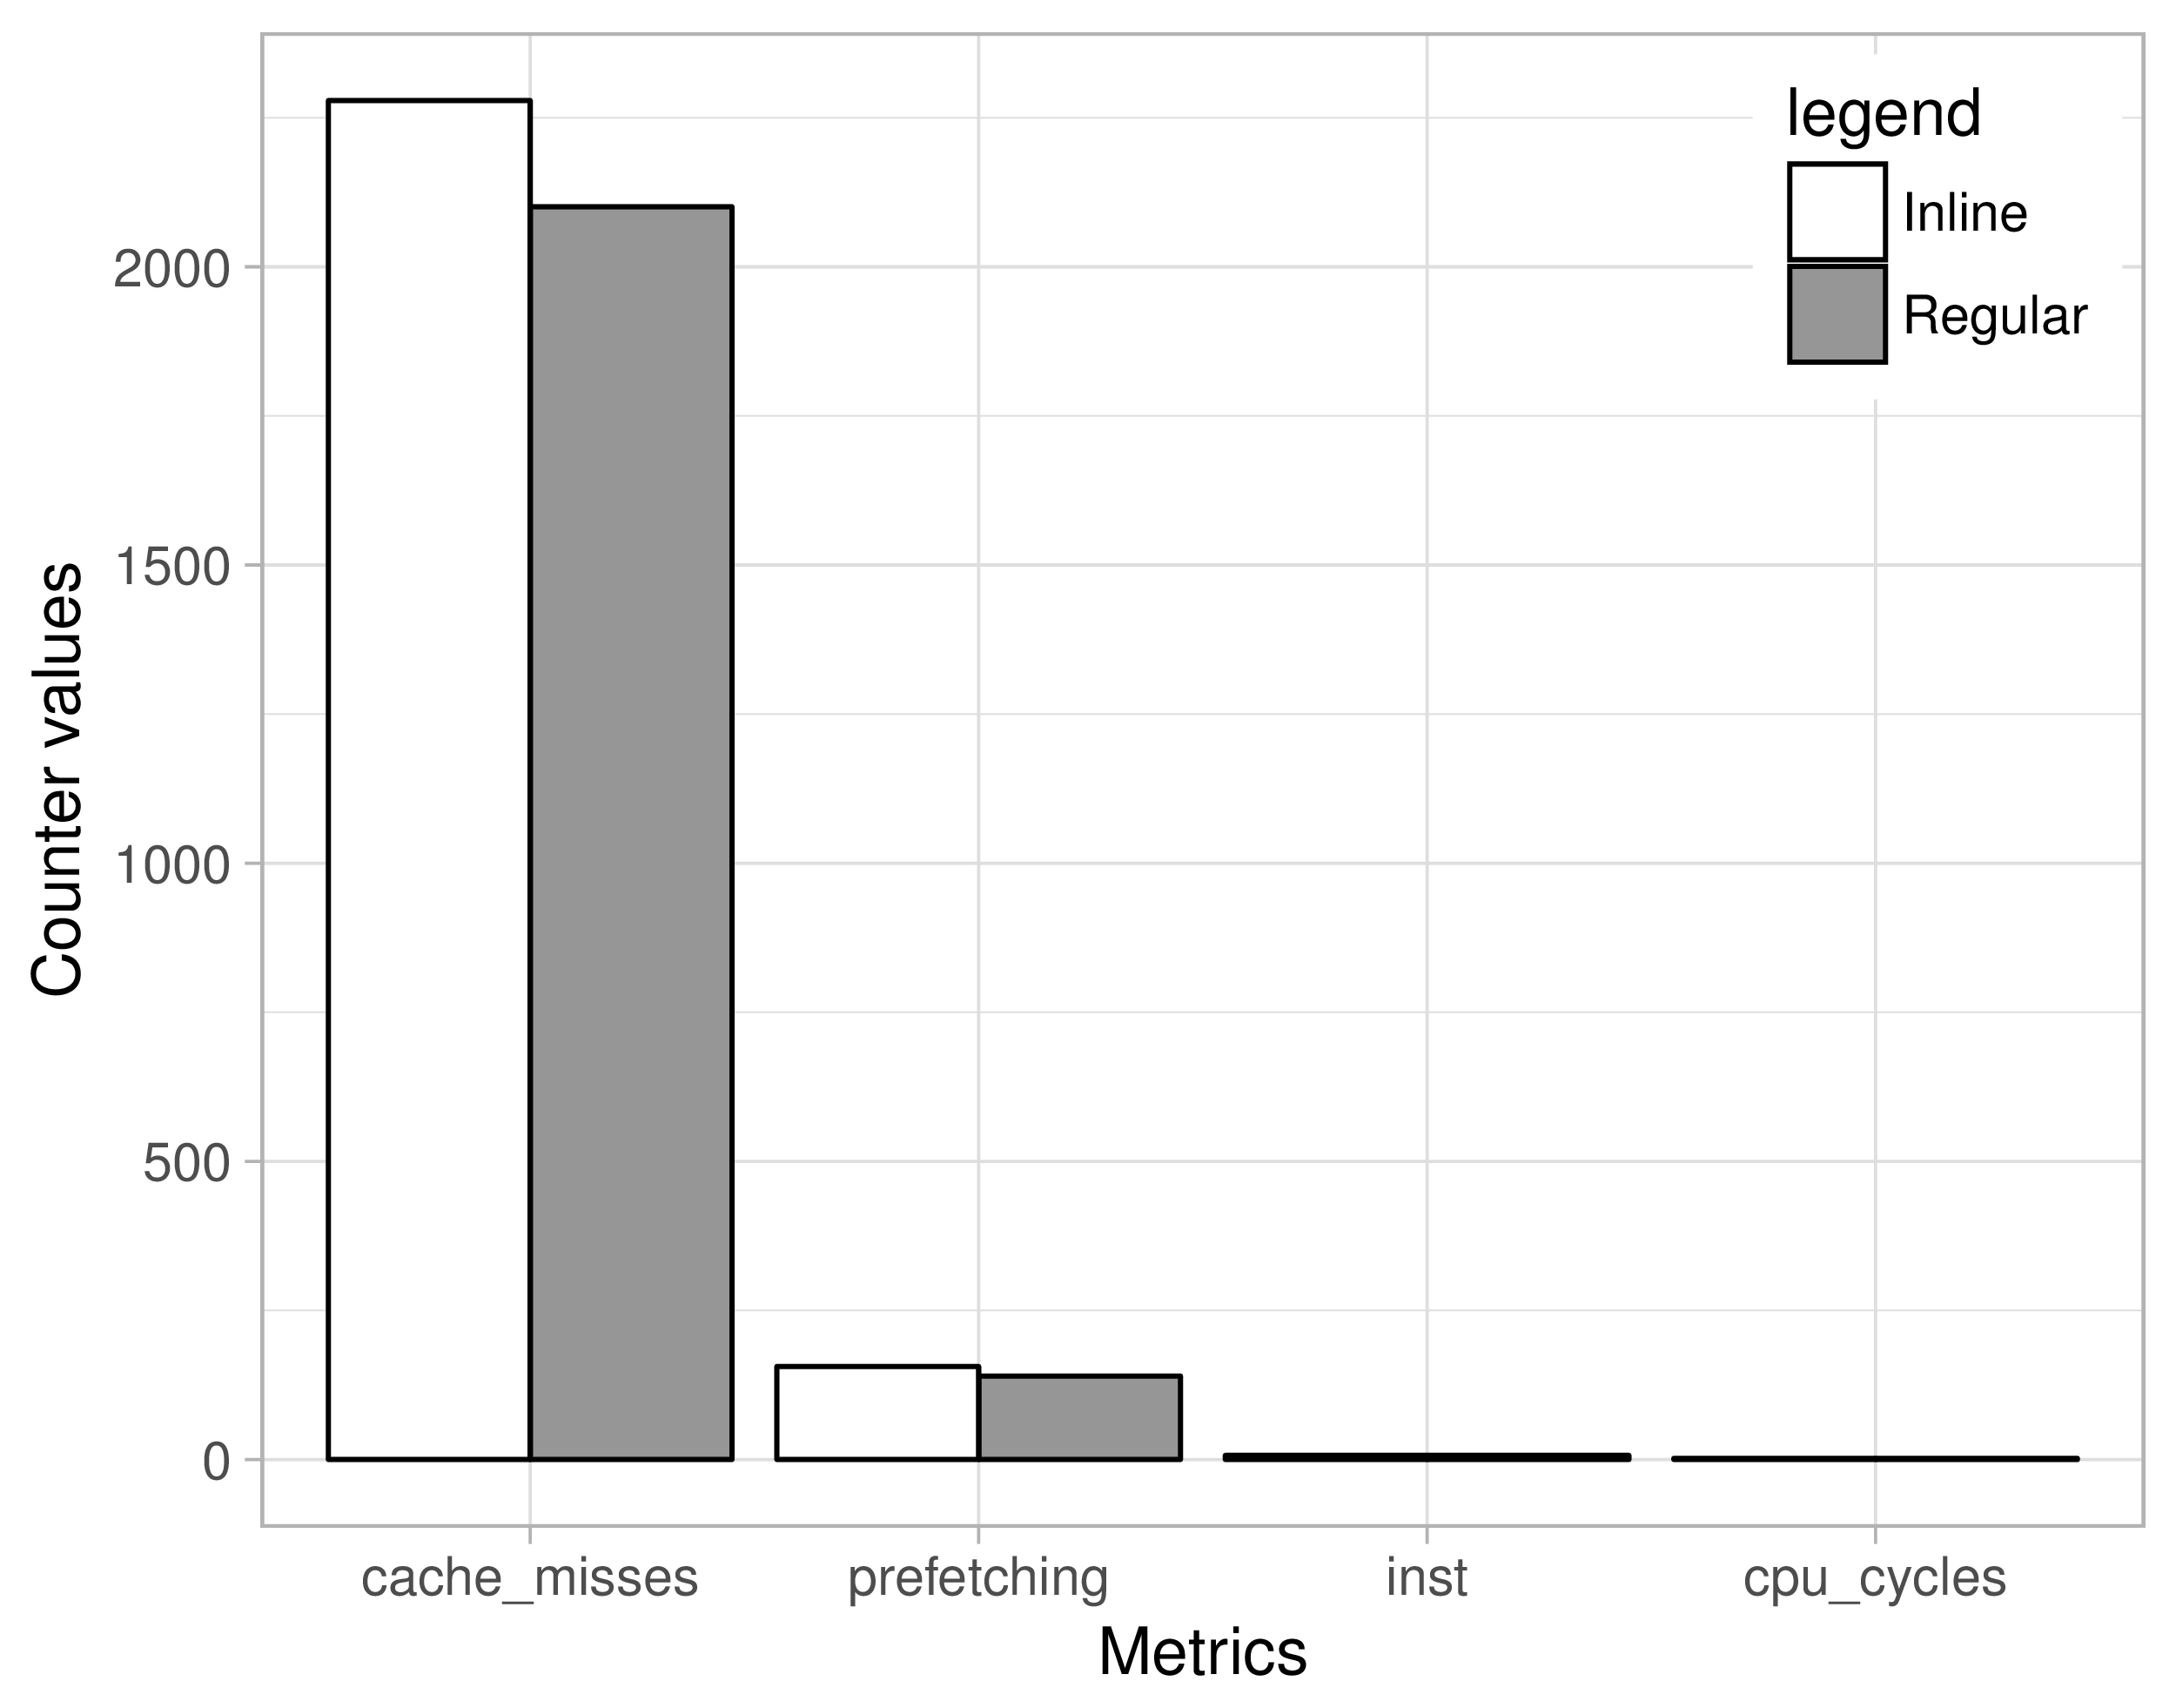
\includegraphics[width=0.57\textwidth]{figures/barplots-inline-vs-regular-counters.png}
        \caption{Distribution of Inline vs Regular functions using String and Integer as return types}
        \label{fig:inline}
    \end{figure}
    
    
    \section{Illustrative Example}
    
\textbf{Open Close}
    To illustrate the approach used, we developed a small code which does several times the process of opening a file subsequently. The code was instrumented with -finstrument functions and this gave the possibility to run the code using Lttng-UST.
    When execute this code several times, some executions have a different behaviour, which we call outliers.
    Using our approach, first we record the executing metrics of the program, then the automated cluster technique is applied, finally we compare the groups: slow executions and fast executions. We deduced that the problem was related with the wait-cpu time metric on the slow executions.
    
    The figure \ref{fig:group} demonstrates the grouping mechanism, which segregated the executions in two groups, the association rule related all the slow executions with wait-cpu group 2 and the fast executions with wait-cpu group 1. The association showed that the wait-cpu was the cause for this difference of the groups.
    
     \begin{figure}[h]
      \centering
        % 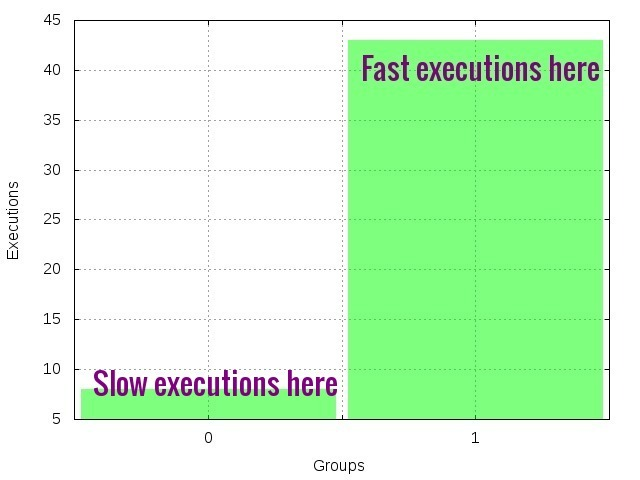
\includegraphics[width=0.50\textwidth]{figures/grouping.jpg}
        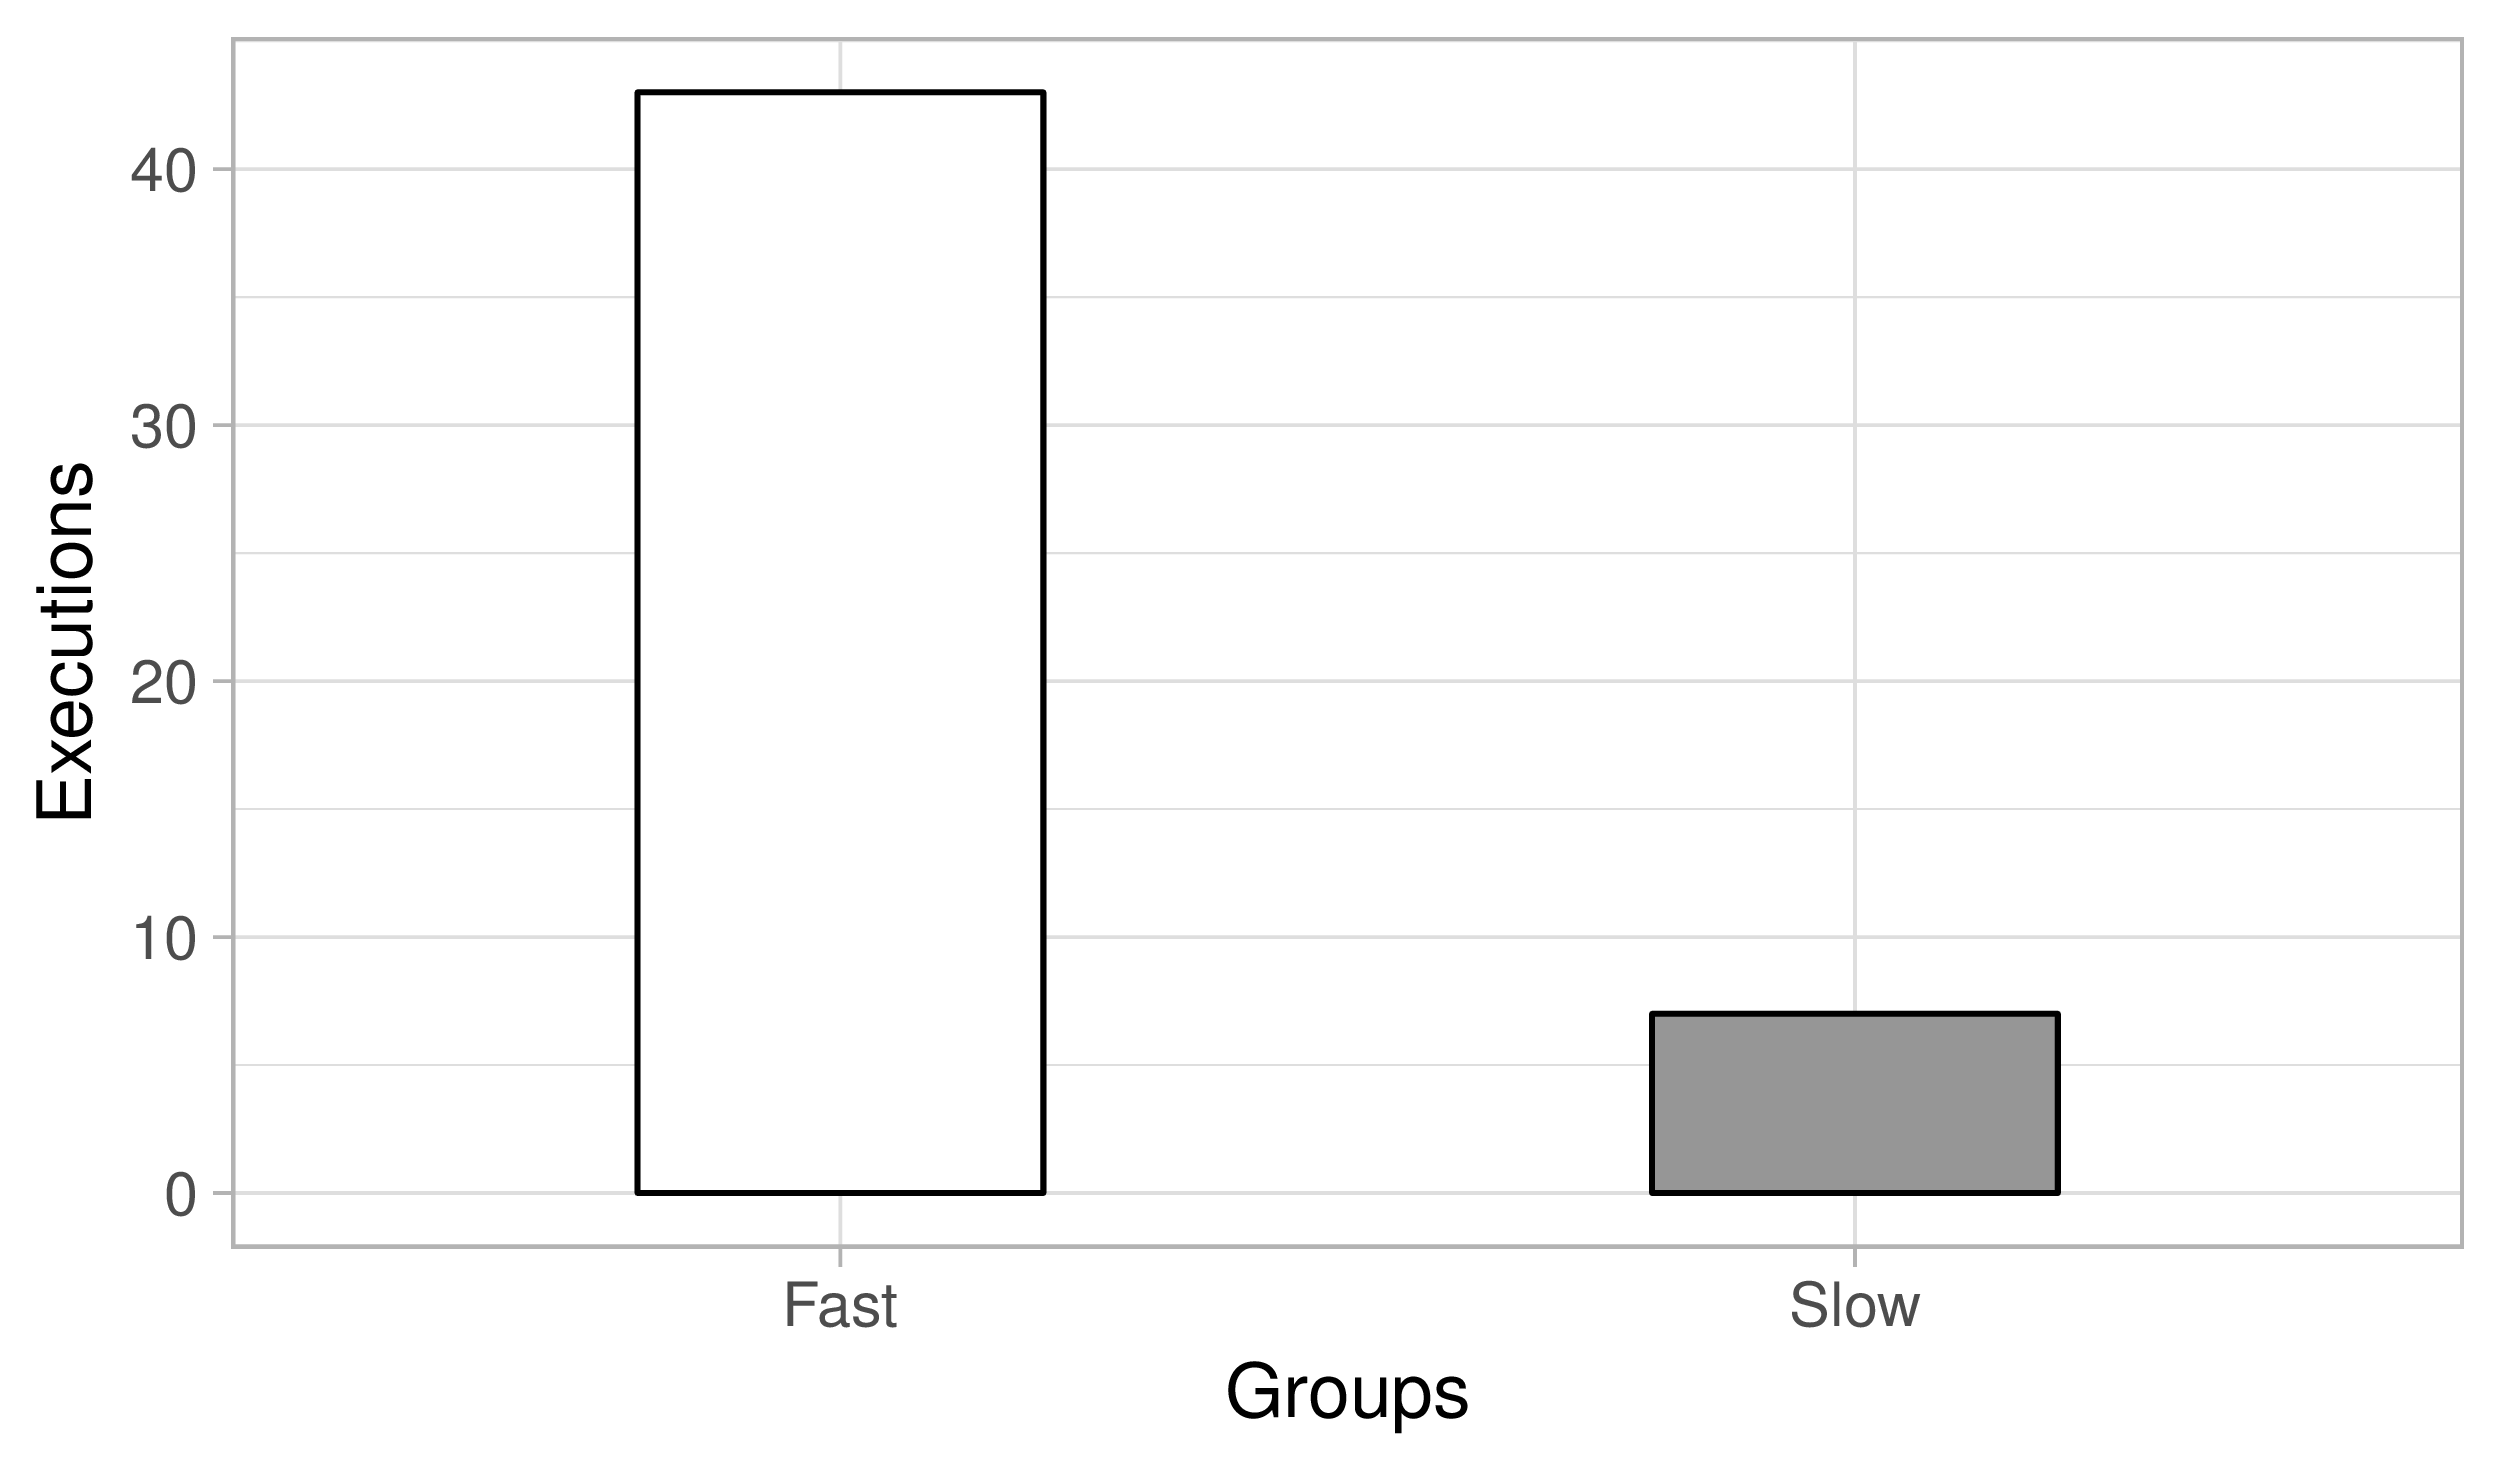
\includegraphics[width=0.65\textwidth]{figures/open-program-groups.png}
        \caption{Comparing executions of Open program}
        \label{fig:group}
    \end{figure}

    
    
\textbf{Executions}
    All experiments were done in a computer with a quad-core Intel® CoreTM i7-3770 CPU running at 3.4 GHz, 16 GB of DDR3 memory and a 7200 RPM hard drive. The Linux kernel version was 3.13.0-49 while the LTTng version was 2.6.0.
% \subsection{\textbf{Scheduler Interference}}
  
% \subsubsection{Summary}
%     A process is executed with lower priority than another, which is triggered on regular intervals. The scheduler plays its role to change the process order at regular times on Linux systems.
    
% \subsubsection{Approach}
%     Our approach was to run the process several times to trigger the conflict with a task with higher priority. While running it, we recorded the tracing data. Then, we executed our clustering analysis and classified the data in several groups. Were able to find that on the fast runs the execution took: x milliseconds. However, on not normal executions - slow executions.
    
% \subsubsection{Results}
%      Were able to find that on the fast runs the execution took: x milliseconds. However, on not normal executions - slow executions. The automated comparison showed that the main difference was on the x function.

    

% \subsection{\textbf{Regression Comparison}}
    
% \subsubsection{Summary}
%     A new feature was added on the new software version and the performance regressions tests are showing a slightly performance difference with a feature, which uses inline functions.
    
% \subsubsection{Approach}
%     Our approach was to run the software several times with the function using and not using inline. The tool was applied from the tracing data. The benchmarks used showed that strings operations with inline can have a difference performance.
    
% \subsubsection{Results}
%     The functions using inline were a little worst in terms of performance to non inline versions. The classification result showed that inline were related with a larger number of cache misses indeed.

%     Figure \ref{fig:case1}, shows the grouping results relating the cache misses with the slow executions groups.
    
%     \begin{figure}[h]
%           \centering
%             \includegraphics{figures/inline.png}
%             \caption{Case study Regression - showing differences on the runs using inline functions and not inline}
%             \label{fig:case1}
%     \end{figure}


\section{Case Studies}
\label{sec:usecases}
We used our approach on the following use cases:

\subsection{Regression Comparison}
    
\subsubsection{Summary}
    A software company is releasing its new version of software with several new features. The performance regressions tests did not find problems and the unitary tests were accepted. Some weeks after the release, the users started to complain about performance issues in one of the features.
    
\subsubsection{Approach}
    Our approach was to run the software several times on the previous and in the current version of the software. Then classified the data using our approach in slow and fast executions. 
    
    \begin{figure}[h]
      \centering
        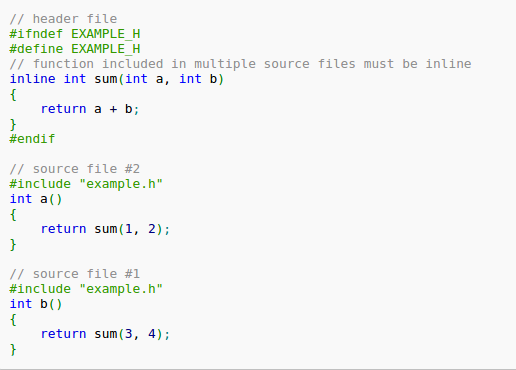
\includegraphics[width=0.50\textwidth]{figures/inline_example.png}
        \caption{Example of Code for inline}
        \label{fig:caseOpt}
    \end{figure}

\subsubsection{Results}
    Were able to find that in-line function addition on the feature increased the number of cache misses and therefore increased the elapsed time of this application. On the source code the in-line functions could be seen as difference although the developers thought that this would improve and not decrease the performance.
    
    Using a comparative approach of the groups we could see the difference of the metrics withing them. Comparing the groups of in-line functions and the groups without inline, we verified that the inline groups comparatively to their respective groups of non-inline, had a significant amount of cache misses. Concluding that cache misses was the essence of the differences.
    
    Table \ref{tab:table}, shows the grouping results relating the cache misses with the slow executions groups comparatively. 
    
\begin{table}[]
\centering
\caption{Table Performance}
\label{tab:table}
\begin{tabular}{ll}
\hline
\multicolumn{2}{c}{Executions}                        \\ \hline
Fast group                & Slow group                \\ \hline
mean of 2500 cache misses & mean of 6500 cache misses
\end{tabular}
\end{table}

\subsection{Page Faults Interference}
    \subsubsection{Summary}
    A program executes several times the process of writing on the buffer, the process reveals a problem after several sub-sequential executions.
    
\subsubsection{Approach}
    Our approach was to run the process several times to trigger this problem. The mechanism classified the executions according to the execution time and also for the metrics.
    
\subsubsection{Results}
     The tree generated had branches with fast and slow executions, 
     The classification was done within the branches of the tree and we were able to find that for all the fast executions (group fast on elapsed time), the group of page-faults were in the first group. On the slow executions, the page-faults were classified on another group. So, the tool revealed the association, and we can conclude that the program triggers more page faults specifically after several executions.\\
     The company was not able to track this problem before because of the prefetching algorithms influence of the executions. This technique is used on the microprocessor architecture to speedup the instructions. The Figure \ref{fig:case1}, is a CCTView result that shows this  difference on the runs on several runs.
    
    \begin{figure}[h]
          \centering
            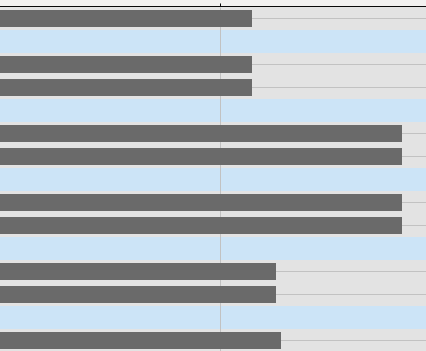
\includegraphics[width=0.50\textwidth]{figures/showing_diff.png}
            \caption{Case study Regression - Tree details showing significantly differences on the runs, where the faster are smaller and the slower are bigger in the images}
            \label{fig:case1}
    \end{figure}
    % Figure \ref{fig:case3}, shows the grouping results relating the page-faults grouping with the slow executions groups.

    
\subsection{Cache Optimization in Server Application}
    
\subsubsection{Summary}
    A server application using a very known content-management framework caches requested data to improve the time access of its content. However, around 1000 requests, the cache is flushed and needs to be redone. So specifically on this request the server will spend more time than on the previous requests.
    
\subsubsection{Approach}
    Our approach was to execute several times a request for a server. While running it, we recorded the tracing data. Then, we executed our clustering analysis and classified the data in several groups.
    
\subsubsection{Results}
    The tree generated by the tool was able to display that on the fast group no time was spent on cache or compile time. However, on slow executions, there was a considerable time spent on compilation time and cache time.
        
    \begin{figure}[h]
      \centering
        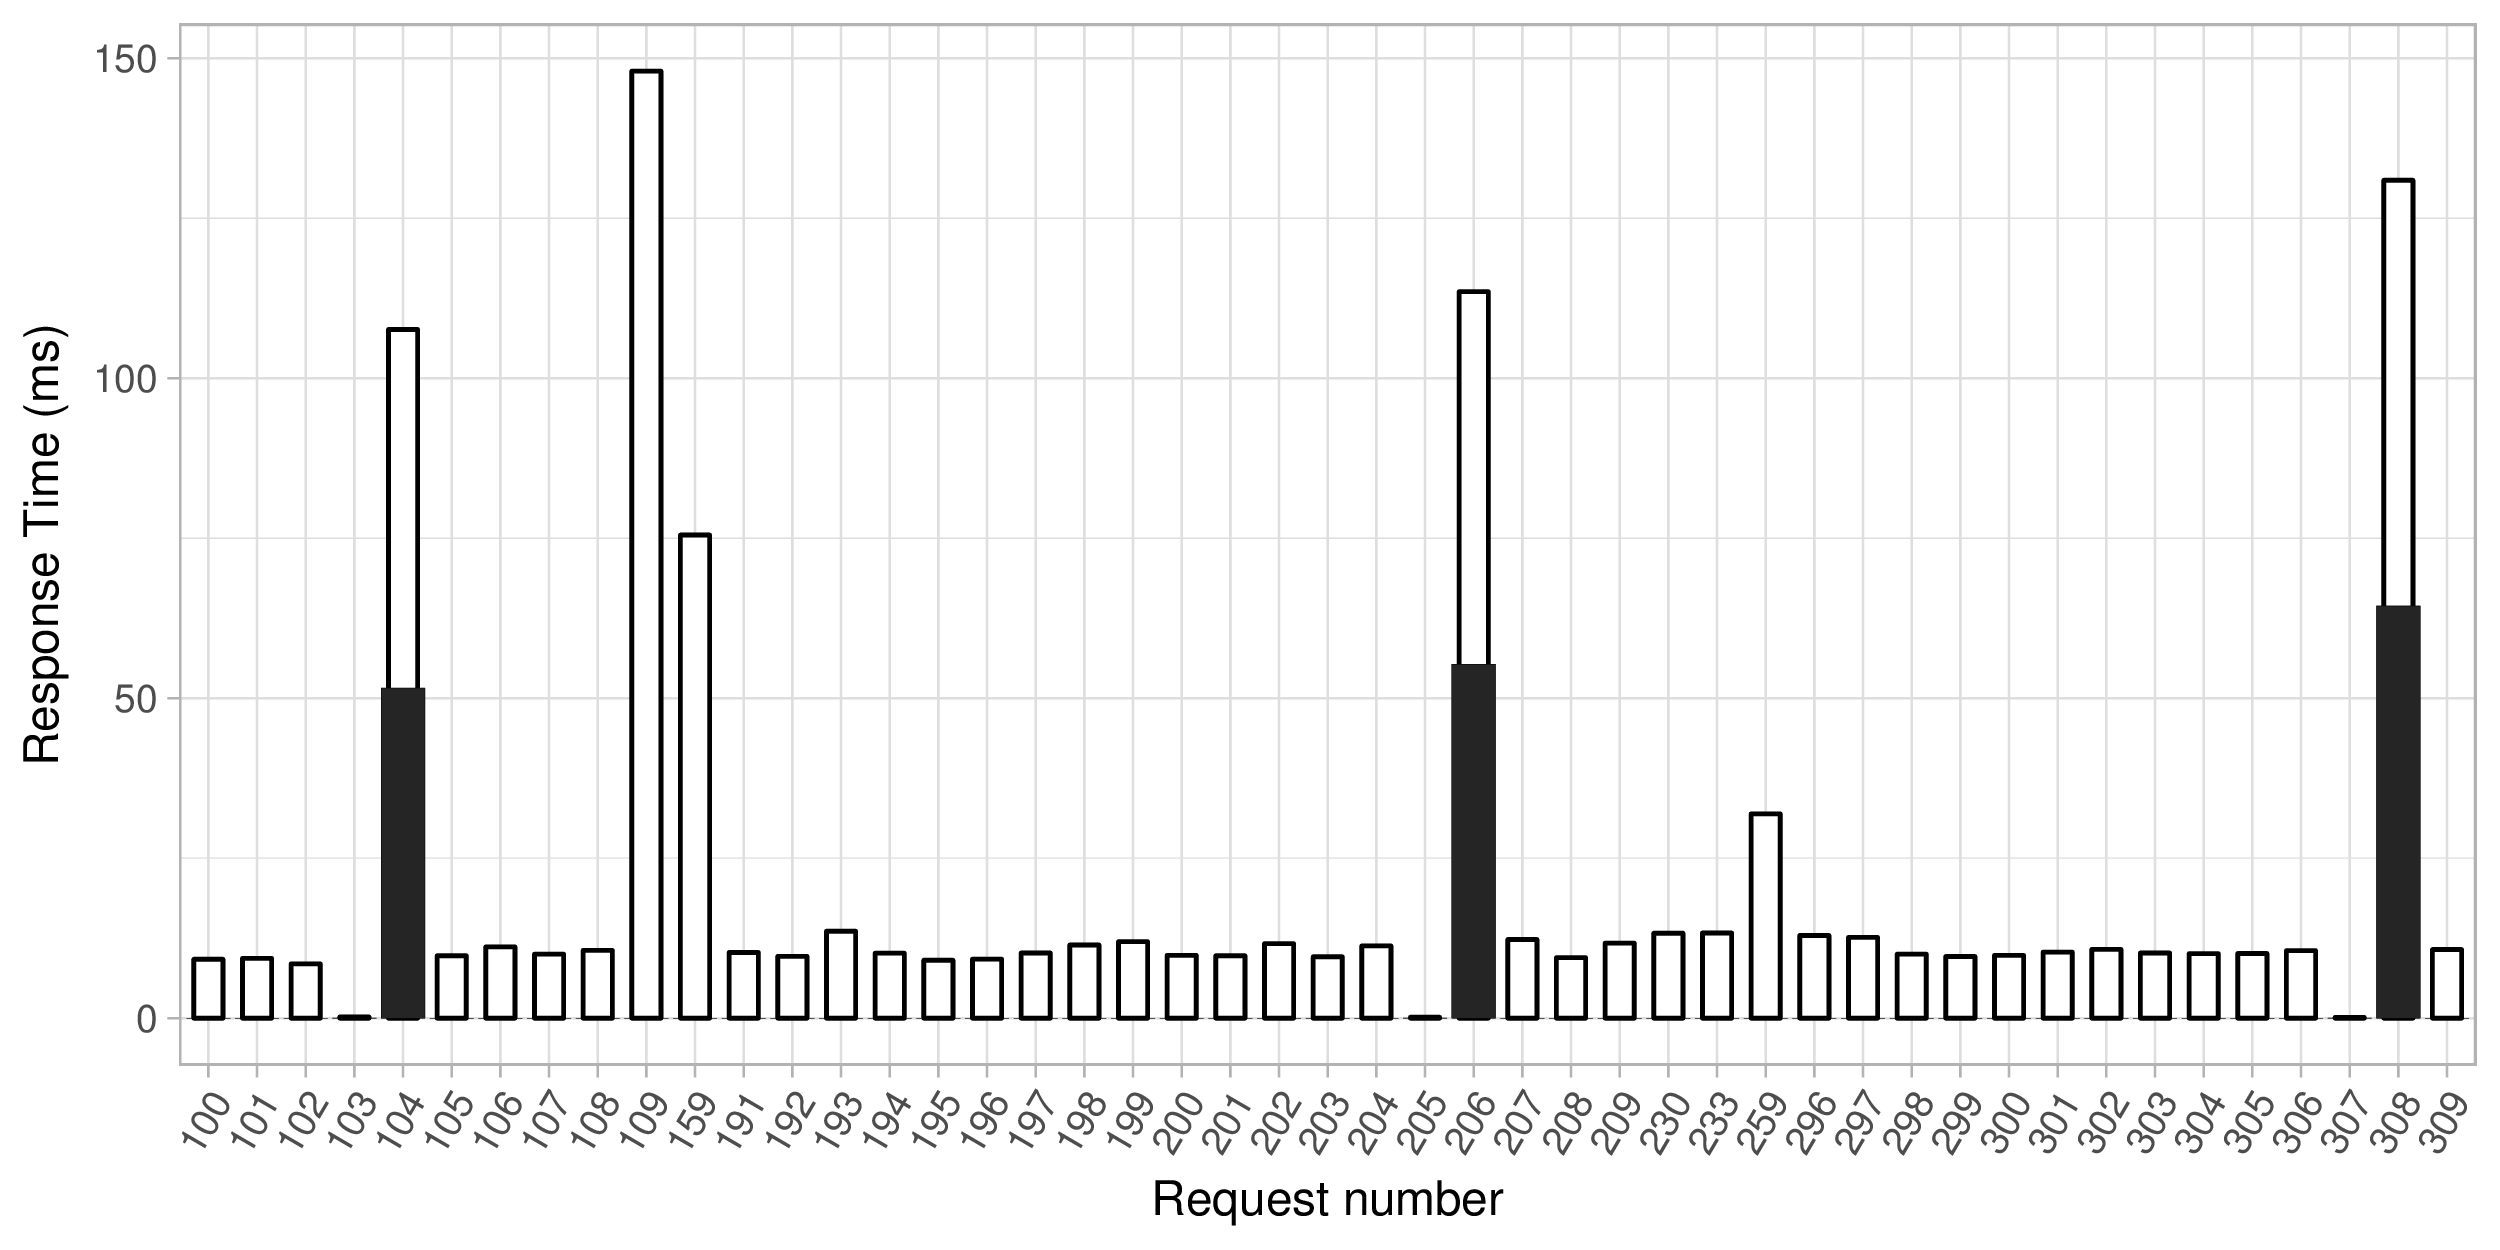
\includegraphics[width=0.50\textwidth]{figures/server-time-series-bar.png}
        \caption{Overhead introduced by I/O for caching on each 100 of requests, The white bat represent the request response time and the dark bar represent the PHP compilation time}
        \label{fig:server-time-series}
    \end{figure}
    % Figure \ref{fig:case4}, shows the grouping results relating the page-faults grouping with the slow executions groups.
    
    
\subsection{Json Cpp}
\subsubsection{Summary}
    JSON is a lightweight data-interchange format. It can represent numbers, strings, ordered sequences of values, and collections of name/value pairs.

    JsonCpp is a C++ library that allows manipulating JSON values, including serialization and deserialization to and from strings. It can also preserve existing comment in unserialization/serialization steps, making it a convenient format to store user input files.
    
    Executing several times the reading from json file, some of the executions have a different time to read those files.    
    
\subsubsection{Approach}
    Our approach was to run the software several times and run the clustering technique then compared the metrics between the groups.
    The auto-grouping technique showed more than 10 groups to be compared, but only a few were taken in consideration.
    
\subsubsection{Results}
    The solution showed differences on the branches of the tree and was able to display the relation with scheduler switches and the performance of this task, this would impact directly on a real task. All the tasks that took more time were related to task scheduling and switches.
    
    
\subsection{OpenCV}
Open Source Computer Vision Library (OpenCV) is an open source computer vision and machine learning software library. This library is used in different problems in computer vision as tracking image. In this section, we will benchmark Optical Flow and HoughLines algorithms, which they are the most evolving features in the recent years.

\subsubsection{Optical Flow} 
The Optical Flow, implemented as Lucas-Kanade algorithm, is an example of method in OpenCV and aims to correlates the apparent motion of objects between two consecutive frames. From some examples of the book \cite{opencv2_book}, this method can be tested with two images and show differences on them. Regressions can be caused by a series of changes on the code. Doing the tests we found a relevant regression on the function Optical Flow.

\textbf{Approach}: Our approach was to run the software several times recording performance metrics using Linux Perf Events. The elapsed time to track the performance is also used in the classification. The runs were related with several versions of OpenCV until find the regression between the versions 2.3.0 and 2.3.1, where the latest version was around 5 times slower than others.

\textbf{Results}: The results correlate the longer duration with more instructions so we could see on the code that a conditional statement was different from version to another, which makes the slower to execute more instructions. This regression was originally reported on \cite{regression_opencv}.
The total number of commits on those two versions were about 250 commits, using this technique, it was able to reduce the difference for about few lines of code and unit tests can be made to trigger specifically this cause after knowing that it is a cache misses problem.

Figure \ref{fig:OpenCV}, shows the result of the optical flow in from two images.
    
\begin{figure}[h]
      \centering
        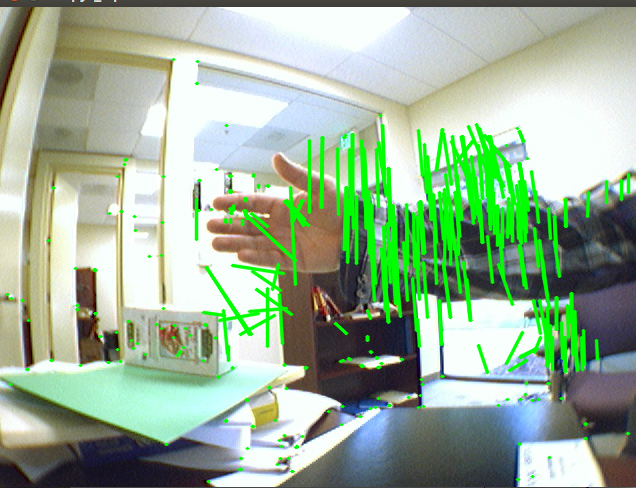
\includegraphics[width=0.50\textwidth]{figures/flow.png}
        \caption{Optical Flow Example}
        \label{fig:OpenCV}
\end{figure}

\subsubsection{HoughLines} 
HoughLines is a line detection mechanism implemented in OpenCV, to find edges in images. This can be used to find edges in roads and it is implemented algorithm is called Canny86. While comparing different versions of opencv, we found that version 3.1 takes more time than version 3.0. in a case of Software Regression, \cite{timeTests}. The source code difference can be found here \cite{opencv_source_diff}.

\textbf{Approach}: Our approach was to run the software several times recording performance metrics using Linux Perf Events in a large file. The elapsed time to track the performance is also used in the classification. The runs were related with several versions of OpenCV until find the regression between the versions 3.1 and 3.0, where the newer version was slower than the previous one.


\textbf{Results}: The results correlate the longer duration associated the longer runs with cache misses. By analyzing the code we were able to find a difference on the file hough.cpp, related with a difference size of the called array. This process reduced the 
    
    Figure \ref{fig:case2}, shows the grouping results relating the cache misses with the slow executions groups.
    
    \begin{figure}[h]
          \centering
            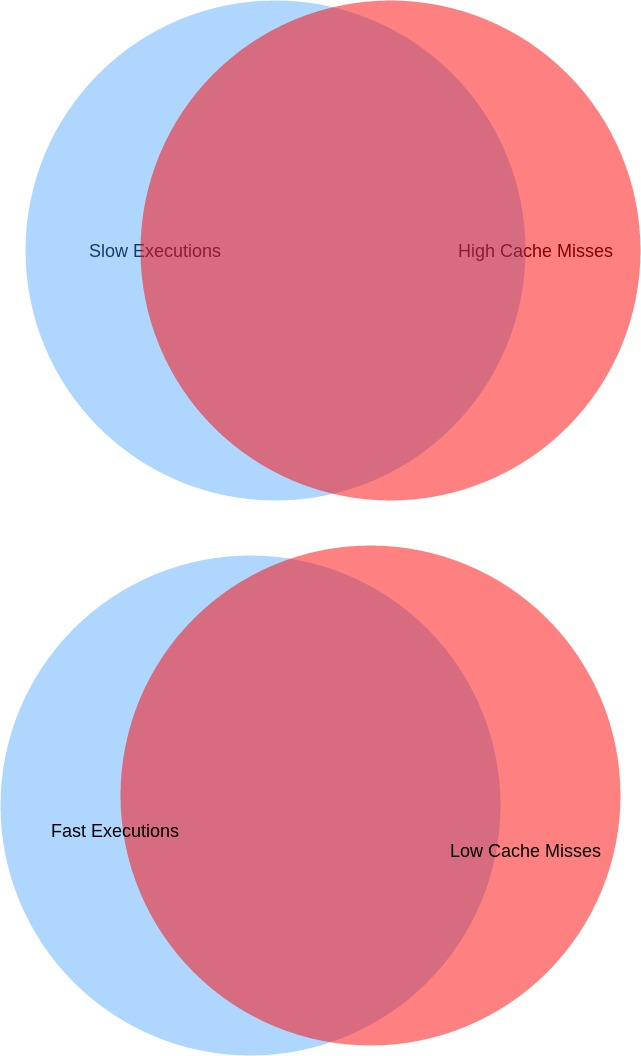
\includegraphics[width=0.350\textwidth]{figures/set_results_cache.jpg}
            \caption{Case study Regression - showing significantly differences in the groups of runs in terms of metrics.}
            \label{fig:case2}
    \end{figure}
    
\subsection{Regression Comparison II}
    
\subsubsection{Summary}
    A software company deployed several new packages in its software including a buffer implementation change. There was a performance impact on this change but it is not possible to track specifically which commit caused the impact. The company would need to run specific Linux commands to find the reason for this problem or reproduce several performance tests with each commit. This scenarios was taken from \cite{essentials} also related to Microsoft bug in \cite{microsoft_bug}.
    
\subsubsection{Approach}
    Our approach was instrument the code and to run the software several times on the previous and in the current version of the software. Then classify the data using our approach in slow and fast executions, although the auto-grouping gave more groups, i.e. reduction of ten to two groups of comparison.
  
\subsubsection{Results}
      The tree generated had branches with fast and slow executions aggregated together. The nodes recorded the several performance metrics including the instructions, cache misses and page-faults.
      We were able to find that page-faults extra addition addition on the feature decreased the performance.
      On the source code, the change on the buffer was an array that was implemented using a row major storage scheme and caused an addition of about 16.384 page faults.
      
      
% \subsubsection{Results}
%      The tree generated had branches with fast and slow executions, 
%      The classification was done within the branches of the tree Figure \ref{fig:case1}, we were able to find that in-line function addition on the feature increased the number of cache misses and therefore increased the elapsed time of this application. On the source code the in-line functions could be seen as difference although the developers thought that this would improve and not decrease the performance.

    The code in highlight shows the difference on the array coding that created the page-faults difference. This code was taken from \cite{essentials}.
    
    % \begin{figure}[h]
    %       \centering
    %         \includegraphics[width=0.2\textwidth]{figures/pf_use_case.png}
    %         \caption{Case study Regression Comparison II - code changes}
    %         \label{fig:caseX}
    % \end{figure}
    
The Figure \ref{fig:k-means} shows the use of k-means with 2 as k number of groups.

    \begin{figure}[h]
          \centering
            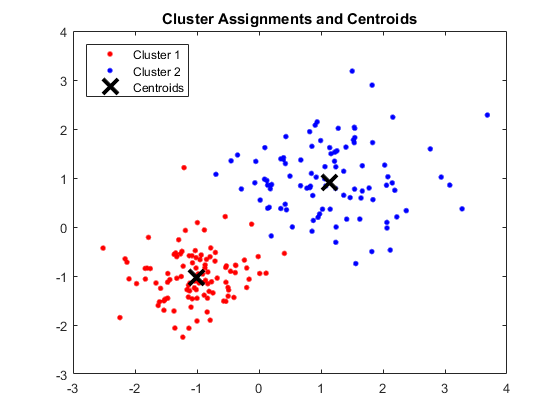
\includegraphics[width=0.50\textwidth]{figures/k-means.png}
            \caption{K-means result}
            \label{fig:k-means}
    \end{figure}
    
    
% \begin{lstlisting}
% #include <stdio.h>
% #define N 10
% /* Block
%  * comment */

% int function1()
% {
%     int i;
%     int i, j;
%     int[128][128];
% }
% \end{lstlisting}

\lstset{language=C++,
                basicstyle=\ttfamily,
                keywordstyle=\color{blue}\ttfamily,
                stringstyle=\color{red}\ttfamily,
                commentstyle=\color{green}\ttfamily,
                morecomment=[l][\color{magenta}]{\#}
}
\begin{lstlisting}

    //Considering 128 words/page\\
    
    int i, j;\\
    int[128][128]; \\
    // original version\\
    for(i = 0; i < 128; i++)\\
        for(j = 0; j < 128; j++)\\
            data[i][j] = 0;\\
    // new version\\
    for(j = 0; j < 128; j++)\\
        for(i = 0; i < 128; i++)\\
            data[i][j] = 0;\\

\end{lstlisting}
% \label{pseudo:page-faults}
% 
% \caption{Case  study   Regression  Comparison   II  -  codechanges}
 


\section{Discussion}
\label{sec:results}
% Present the results for your research questions. For each one, provide a short motivation (why is this question important to answer?), brief overview of analyses used (of those discussed in \autoref{sec:approach} and your actual results. For each individual result of a research question, put a first sentence in bold, then use the rest of the paragraph and possibly follow-up paragraphs to explain the result. Do this for each result of a question, and all questions.

This section presents a discussion related with the research questions presented on the introduction, as well as, the solution presented. The results of the use cases clarifies the research questions delimited on the introduction and conduct new insights on this performance part.

\begin{itemize}

\item RQ 1: How can we build an efficient and flexible model for performance comparison?\\
    Using the enhanced calling context tree it is possible to aggregate performance metrics and compare executions efficiently. The CCT can be built with or without source code modification. The possibility to build it without source code brings the opportunity to analyze the dynamic structure and an accurate behaviour can be used.\\
    
\item RQ 2: Is it possible to automate the performance analysis?\\
    Our work demonstrated the possibility to use non-supervised machine learning methods to compare and find performance problems, specifically using a comparative heuristic technique. The approach used is to use a comparative clustering mechanism, which can efficiently separate the data for a realistic comparison.\\
    
\item RQ 3: How accurate was the obtained results?\\
    The methodology used was able to find association between groups of metrics and consequently associate the cause of elapsed time variations. However this approach can have type I or type II errors - false positives and false negatives.
    
\end{itemize}

% The solution presented was able to automate the process of clustering by using a deterministic heuristic comparison.



\section{Threats to Validity}
\label{sec:validity}
This section discusses the threats to the validity of our study.\\
\textbf{Time analysis}
    Our approach is based on comparing several clusters to take the best according to the SSE, which requires a comparatively long period of time. Our study aims to use an automated non-supervised clustering method, thus the analysis time is a minor factor if it is less than human analysis. Although the analysis required just a few minutes between building the ECCT tree and the classifying the metrics. Another highlights is that the analysis is made offline, so the time will not influence on the performance of the software and does not require stopping the software development.
    
\textbf{Quantity of groups}
    Considering the automated heuristic used can give a high number of groups for evaluation. This process can increase the difficult for evaluation.

\section{Conclusion}
\label{sec:conclusion}
% In conclusion, this research developed a solution that showed the possibility to use clustering mechanisms without a human intervention to find causes of performance problems. As a contribution for developers, this  paper  introduces  the  visualization  tool  for  the  Calling Context Tree with Flame Graphs and Auto Cluster mechanisms. \\
% The clustering data was built through a bottom-up analysis on collected stack traces, from recorded tracing data on ECCTs. This data structure, was implemented in the CCT View inside TraceCompass framework and provides several run-time properties of the studied software.\\
% % The implementation also developed the RGG differential flamegraph to compare groups of executions. This implementation uses a three colors: red, green and gray, which is a different approach of the original work, but was done to avoid ambiguity between slower executions and equal time executions.
% The solution presented an automated algorithm done with an heuristic comparison. This approach is the first one to be done on performance analysis on trace executions and call graph data. The solution also presented a flexible approach which can be used combined with different means to collect the data, as LTTng and Perf counter to form the data that will be analyzed, as was done in some use cases.
% The grouping approach used was used  without supervision. This is an advantage over techniques that require training phase. For example, Support Vector Machines, which require data pre-classification. \\

% This paper also did a comparison among the possible techniques that can be used for this kind of operation. In the comparison the techniques that were non-supervised required another level of data treatment, for example the SVM technique, and therefore can be overpassed by the auto clustering technique, suggested here.

% Our work was able to find causes of performance issues without human intervention and can be applied to other cases to find other problems. The implementation as part of the TraceCompass framework aims to apply this approach for more cases and large scale software analysis.

% As future work, we plan to expand our investigation by using non-linear models to track regression problems in different software versions, as investigated in \cite{deep}. This can be used as an automated test to find software regressions. An example of possible models are feed-forward network, \cite{deep}, also called deep learning networks.
% The models need to be able to characterize specifically non-linear dependencies and be able to be used without non label data. Considering those restrictions, an Autoencoder or a Restricted Boltzmann Machine are also candidates.\\ 
% %This require modifications in the loss function.

% Another possibility would be to apply other techniques such as Apriori algorithm as described in \cite{apriori}, which can determine association rules among the metrics recorded in the enhanced CCT, for each cluster. Finally, tracking performance issues before the release of new software is an interesting path to be followed. Thus, an automated mechanism to find them before the release of a new version of software is very promising. A possibility could be to develop a mechanism to be executed as a regression test suite, from the machine learning models described above, before the releasing.

In conclusion, this research developed a solution that showed the possibility to use clustering mechanisms without a human intervention to find causes of performance problems. As a contribution for developers, this  paper  introduces  the  visualization  tool  for  the  Calling Context Tree with Flame Graphs and Auto Cluster mechanisms. \\
The clustering data was built through a bottom-up analysis on collected stack traces, from recorded tracing data on ECCTs. This data structure, was implemented in the CCT View inside TraceCompass framework and provides several run-time properties of the studied software.\\

% The implementation also developed the RGG differential flamegraph to compare groups of executions. This implementation uses a three colors: red, green and gray, which is a different approach of the original work, but was done to avoid ambiguity between slower executions and equal time executions.

The solution presented an automated algorithm done with an heuristic comparison. This approach is the first one to be done on performance analysis on trace executions and call graph data. The solution also presented a flexible approach which can be used combined with different means to collect the data, as LTTng and Perf counter to form the data that will be analyzed, as was done in some use cases.

The grouping approach used was used  without supervision. This is an advantage over techniques that requires training phase. For example, Support Vector Machines, which require data pre-classification. \\

This paper also did a comparison among the possible techniques that can be used for this kind of operation. In the comparison the techniques that were non-supervised required another level of data treatment, for example the SVM technique, and therefore can be overpassed by the auto clustering technique, suggested here.

Our work was able to find causes of performance issues without human intervention and can be applied to other cases to find other problems. The implementation as part of the TraceCompass framework aims to apply this approach for more cases and large scale software analysis.


\section{Acknowledgement}
\label{sec:acknowledgement}
The author would like to thanks the Council of Research of Canada and the Dorsal lab. 

 